\documentclass[10pt,twocolumn,letterpaper]{article}

\usepackage{iccv}
\usepackage{times}
\usepackage{epsfig}
\usepackage{graphicx}
%\graphicspath{{/Users/JohnsonJohnson/Downloads/ReIDCodes/Figures/}{../pdf/}{../jpeg/}}
%\DeclareGraphicsExtensions{.pdf,.jpeg,.png}
\usepackage{amsmath}
\usepackage{amssymb}
\usepackage{float}
\usepackage{bm}
\usepackage{booktabs}
\newcommand{\bftab}{\fontseries{b}\selectfont}

% Include other packages here, before hyperref.

% If you comment hyperref and then uncomment it, you should delete
% egpaper.aux before re-running latex.  (Or just hit 'q' on the first latex
% run, let it finish, and you should be clear).
\usepackage[pagebackref=true,breaklinks=true,letterpaper=true,colorlinks,bookmarks=false]{hyperref}

% \iccvfinalcopy % *** Uncomment this line for the final submission

\def\iccvPaperID{****} % *** Enter the ICCV Paper ID here
\def\httilde{\mbox{\tt\raisebox{-.5ex}{\symbol{126}}}}

% Pages are numbered in submission mode, and unnumbered in camera-ready
\ificcvfinal\pagestyle{empty}\fi
\begin{document}

%%%%%%%%% TITLE
\title{Person re-identification based on kernel local Fisher discriminant analysis and Mahalanobis distance learning}

\author{Qiangsen He\\
University of Ottawa\\
Ottawa, Ontario\\
{\tt\small firstauthor@i1.org}
% For a paper whose authors are all at the same institution,
% omit the following lines up until the closing ``}''.
% Additional authors and addresses can be added with ``\and'',
% just like the second author.
% To save space, use either the email address or home page, not both
\and
Second Author\\
Institution2\\
First line of institution2 address\\
{\tt\small secondauthor@i2.org}
}

\maketitle
%\thispagestyle{empty}


%%%%%%%%% ABSTRACT
\begin{abstract}
   In person re-identification (Re-ID), robust descriptors and metric are essential to improve accuracy. Mahalanobis distance based metric learning is a popular method for metric learning. However, for descriptors with high dimensionality (thousands or more), it is intractable to learn a high dimensional semi-definite positive (SPD) matrix without dimension reduction.  Many metric learning methods have been proposed to learn a subspace that preserves those discriminative information. However, few works have been done to study metric learning on those subspaces obtained after an initial dimension reduction. In this paper, a two-level structure of metric learning is proposed. The kernel local Fisher discriminant analysis (KLFDA) is used to reduce dimension taking advantage of the idea that kernelization method can greatly improve Re-ID performance \cite{KernelVersionMetrics}. Then a Mahalanobis distance metric is learned on the lower dimensional descriptors based on the constraint that the intraclass distance must be at least one unit smaller than the minimum interclass distance. By comparing the intraclass distance only with the minimum interclass pair the computation complexity of metric learning is reduced. This method turns to have state-of-the-art performance compared with other advanced metric learning methods.
\end{abstract}

%%%%%%%%% BODY TEXT
\section{Introduction}

% no \IEEEPARstart
Person re-identification (Re-ID) has received increasing attention in recent years. Re-ID is very challenging due to several factors such as low image resolution, occlusion, background noise and different camera color responses. In the single-shot Re-ID problem, where only one image is provided in each camera for each person, confusion often occurs when different people have similar pose or clothes (shown in Figure \ref{fig::SimilarInterC}). In the multi-shot case, there might exist significant difference even in different frames of the same person showing different pose and illuminations (shown in Figure \ref{DisimilarIntra}). To overcome these challenges most previous works either try to find better feature representation \cite{LOMO, GOG, RegionCovariance, SDALF} or learn better metrics \cite{KISSME, LFDA, PCCA, TDL, PRDC, LMNN, KLFDA, KCCA, KernelVersionMetrics, NFST, ITML}. A good descriptor is supposed to be robust to illumination change and occlusions. Though much progress has been made, there still exists some challenges caused by classical problems like small sample problem (SSS) and high computation complexity on large datasets.
\begin{figure} 
\centering
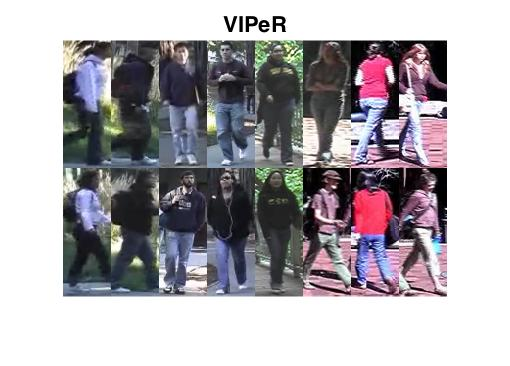
\includegraphics[width=0.8\linewidth]{SimilarInter.jpg}
\vspace{-2em}
\caption{Different pedestrians may look the same under the same viewpoint when wearing similar clothes and have similar postures. In this figure, individuals in each column are different while they look the same under the same viewpoint.}
\label{fig::SimilarInterC}

\end{figure}

\begin{figure} 
\centering
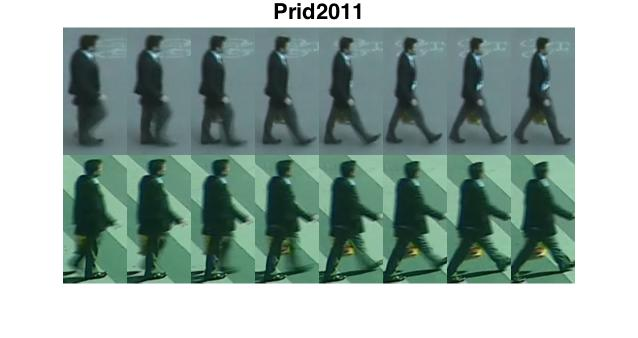
\includegraphics[width=1\linewidth]{DisimilarIntra.jpg}
\vspace{-2em}
\caption{Pedestrians may look different under different angle, illumination and postures. In this figure, images in the first and second row are of the same person under different viewpoints and posture.}
\label{DisimilarIntra}
\end{figure}
%Metric learning 
%\indent Among all those metric learning methods, Fisher discriminant analysis (FDA) proves to be one of advanced metrics to improve Re-ID performance. It tries to maximize the ration of interclass scatter matrix versus intraclass scatter distance and this problem is transformed as a eigenvalue decomposition problem. Local Fisher discriminant analysis combines locality preserving projection (LPP) with FDA to exploit locality of sample points. Besides, kernel method \cite{KernelVersionMetrics} has been shown to improve Re-ID performance since it exploits the nonlinearity of data.\\
\indent For descriptors with high dimensionality, it is hard to directly learn an SPD matrix $\bm{M}$ when the small sample size $n (n<<d)$ is small. A popular method is to use principal component analysis (PCA) to reduce dimension. PCA is very popular for dimensionality reduction, but PCA is a global dimension reduction scheme. As a result, much interclass discriminative information will be lost after dimensionality reduction. In this paper kernel local Fisher discriminant analysis (KLFDA) \cite{KernelVersionMetrics} is used to reduce dimensionality, this supervised dimension reduction combines the linear discriminant analysis and locality preserving projection. Moreover, the kernelization version of LFDA proves to improve performance and reduces computation cost. However, the use of metric learning on dimensionality reduced vectors by KLFDA hasn't been fully studied.\\
\indent The contributions of this paper are as follows. (1) KLFDA and metric learning are combined together to improve Re-ID performance. Previous works mainly used KLFDA  \cite{KernelVersionMetrics} as a subspace learning method. Euclidean distance is then used to measure the similarity of dimension reduced descriptors. (2) Inspired by \cite{TDL}, we propose to learn a Mahalanobis distance matrix based on the constraint that intraclass distance is at least one unit smaller than the minimum interclass distance. Therefore, metric learning in the lower dimensional space is transformed into an optimization problem solved by an iterative process using gradient descent method. Here we compare the intraclass distance only with the minimum interclass distance in each iteration thus avoiding the need to compute every possible possible positive and negative pairs. Extensive experiments are performed on VIPeR, CUHK01, prid\_450s and GRID dataset. These ones demonstrated that the proposed method can produce state-of-the-art performance on some of these datasets.

%-------------------------------------------------------------------------

\section{Related work}
Descriptor design and metric learning are two core components in people Re-ID. In descriptor design, color, texture and their statistical properties are exploited to characterize individuals. In \cite{SDALF} Symmetry-Driven Accumulation of Local Features (SDALF) divides the human silhouette into head, torso and legs and extract features according to their symmetry and asymmetry axis. In \cite{LOMO} Local Maximal Occurrence (LOMO) uses overlapping samplings and creates local histograms of pixel features extracting maxima value along horizontal stripes. In \cite{GOG} hierarchical Gaussian descriptor constructs a two-level model from pixel features to patch features and from patch features to region features.\\
\indent For metric learning,  \cite{LOMO} represents the within-class and between-class difference individually with a Gaussian model. The problem to distinguish different classes is transformed into maximize the probability ratio of between-class and within-class Gaussian distribution. In \cite{NFST} Null Foley-Sammon transform (NFST) is proposed to find a null space so that with this space the intraclass points collapse to a same point in the null space while interclass points are projected to different points.\\
\indent Convolutional neural networks (CNN) have also been exploited in Re-ID. In \cite{RecurrentCNN}, the author proposes a recurrent neural network layer and temporal pooling to combine all time-steps data to generate a feature vector from a video sequence. In \cite{MultiCNN}, the author proposes a multi-channel layer based neural network to jointly learn both local body parts and whole body information from input person images.  In \cite{DeepfeatureCNN}, a convolutional neural network learning deep feature representations from multiple domains is proposed, and this work also proposes a domain-guided dropout algorithm when learning from different datasets. \\
\indent There are many other works based on convolutional neural networks. However, person re-identification may be one of the areas where CNN performance may not perform as well as regular machine learning methods because of the small sample size problem (SSS). In most datasets, the sample size of each pedestrian is quite small. Especially in single-shot Re-ID only one frame is provided in each view for each person. This is why Re-ID more often relies on classical machine learning.\\
\indent In this paper, the Mahalanobis distance learning is motivated by the Top-push Distance Learning method described in \cite{TDL}. An objective function is created based on the constraint that for each within-class person pair the distance should be at least one unit smaller than the minimal between-class person pair distance. This function is then optimized with gradient descent method. But first, dimension reduction is applied to a high-dimensional descriptor.

%% metric learning
\section{Dimension reduction based on kernel local Fisher discriminant analysis }
%\subsection{Background of kernel LFDA}
%The original descriptor has a high dimension and dimensionality disaster will be brought about if the original high-dimensional descriptor is used to learn a metric matrix. One popular method is to reduce the high dimension then learn a metric matrix in the lower dimension data. Among those methods to reduce dimension, principal component analysis is often used. However, PCA is a unsupervised dimension reduction and may have a low performance for those reasons, $(1)$, PCA is to maximize the variance of dimension reduced data, and as a unsupervised method it doesn't has a full consideration of the the relation of between and within classes, it is very likely that the descriptors of different classes can be mixed up in the dimension reduction; $(2)$ PCA may suffer from the small sample size problem. In some Re-ID datasets, there may be two or less images for each pedestrian in each viewpoint (like VIPeR), if the dimension of descriptor is much bigger than sample size, much information can be lost with PCA.

%In this paper the kernel local Fisher discriminant analysis is adopted. This method is a combination of Fisher discriminant analysis[ ] and and the locality preserving projection in [LPP ]. 
KLFDA is the kernel version of local Fisher discriminant analysis (LFDA). For a set of $d$-dimensional observations $\bm{x}_i$, where $i\in\{1,2,\cdots,n\}$, and a set of class labels $l_i\in\{1,2,\cdots,l\}$, two matrix are defined as the intraclass scatter matrix $\bm{S}^{(w)}$ and interclass matrix
$\bm{S}^{(b)}$ as follows,
\begin{equation}
\begin{aligned}
\bm{S}^{(w)} = \mathop{\sum} _{i=1}^l\mathop{\sum}_{j:l_j = i} (\bm{x}_j - \bm{\mu}_i)(\bm{x}_j - \bm{\mu}_i)^T, \\
\bm{S}^{(b)} = \mathop{\sum} _{i=1}^l n_i(\bm{\mu}_i - \bm{\mu})(\bm{\mu}_i - \bm{\mu})^T,
\end{aligned}
\end{equation}
where the $\bm{\mu}_i$ is the mean of samples whose label is $i$, and $\bm{\mu}$ is the mean of all samples,
\begin{equation}
\begin{aligned}
\bm{\mu}_i = \frac{1}{n_i} \sum_{l_j=i} \bm{x}_j, 
\bm{\mu} = \frac{1}{n} \sum \bm{x}_i.
\end{aligned}
\end{equation}

The Fisher discriminant analysis transform matrix $\bm{T}_{FDA}$ can be represented as 
\begin{equation}
\bm{T}_{FDA} = \arg\max_T \frac{\bm{T}^T\bm{S}^{(b)}\bm{T}}{\bm{T}^T\bm{S}^{(w)}\bm{T}}.
\end{equation}
Fisher discriminant analysis minimizes the intraclass scatter matrix while maximize the interclass scatter matrix. $\bm{T}$ is computed through an eigenvalue decomposition and $\bm{T}_{FDA}$ is represented as the set of all the corresponding eigenvectors, as $ \bm{T} = [\bm{\phi}_1,\bm{\phi}_2,\cdots,\bm{\phi}_k]$.

FDA dimension reduction however has poor performance when dealing with multimodal classes. In \cite{LPP} locality preserving projection (LPP) is proposed to exploit data locality. In LPP an affinity matrix is created to record the affinity of sample $\bm{x}_i$ and $\bm{x}_j$.  Typically the range of elements in $\bm{A}_{i,j}$ is $[0,1]$. There are many ways to define a $n \times n$ affinity matrix $\bm{A}$. Usually two sample points at a small distance have a larger affinity value than more distant point pairs. In this case if  $\bm{x}_i$ is within k-nearest neighbours of $\bm{x}_j$ then $\bm{A}_{i,j} = 1$ otherwise  $\bm{A}_{i,j} = 0$.  LFDA combines FDA and LPP and has better performance \cite{KLFDA}. The key in LFDA is it assigns weights to elements in $\bm{A}^{(w)}$ and $\bm{A}^{(b)}$, so that,

%Another diagonal matrix $D$ can be defined that each diagonal element is the sum of corresponding column in $\bm{A}$,
%\begin{equation}
%\bm{D}_{i,i} = \mathop{\sum}_{j=1}^n \bm{A}_{i, j} 
%\end{equation}
%then the LPP transform matrix is defined as follow,
%\begin{equation}
%\bm{T}_{LPP} = \mathop{\arg\min}_{\bm{T}\in\bm{R}^{d\times m}} \frac{1}{2}\mathop{\sum}_{i, j= 1}^n \bm{A}_{i,j} ||\bm{T}^T\bm{x}_i - \bm{T}^T\bm{x}_j||
%\end{equation}
%so that $ \bm{T}^T\bm{X}\bm{D}\bm{X}^T\bm{T} = \bm{I} $.
%Suppose the subspace has a dimension of $m$, then LPP transform matrix $T$ can be represented as 
%
%$$\bm{T}_{LPP} = \{ \bm{\phi}_{d-m+1} | \bm{\phi}_{d-m+1} | \cdots \bm{\phi}_{d}\} $$
%
%And each $\bm{\phi}$ in $T$ is the eigenvector of following fomula,
% \begin{equation}
%\bm{X}\bm{L}\bm{X}^T\bm{\phi} = \gamma\bm{X}\bm{D}\bm{X}^T
%\end{equation}
%where $\gamma$ is corresponding eigenvalue of $\bm{\phi}$, and $L = D - A$.
%But the LPP dimension reduction is still not discriminant enough, 


\begin{equation}
\begin{aligned}
\bm{S}^{(w)} = \frac{1}{2}\sum _{i=1}^l\sum_{j:y_j = i} \bm{A}_{i,j}^w (\bm{x}_j - \bm{\mu}_i)(\bm{x}_j - \bm{\mu}_i)^T, \\
\bm{S}^{(b)} =  \frac{1}{2}\sum _{i=1}^l \bm{A}_{i,j}^b(\bm{\mu}_i - \bm{\mu})(\bm{\mu}_i - \bm{\mu})^T,
\end{aligned}
\end{equation}
where 
\begin{equation}
\begin{aligned}
\bm{A}_{i,j}^{(w)} = \left \{ 
\begin{array}{rcl}
\bm{A}_{i,j}/n_c &  &y_i = y_j \\
0 & & else
\end{array}
  \right., \\
  \bm{A}_{i,j}^{(b)} = \left \{ 
\begin{array}{rcl}
(\frac{1}{n} - \frac{1}{n_c})  \bm{A}_{i,j} &  &{y_i = y_j }\\
\frac{1}{n} & & {else}
\end{array}
  \right..
 \end{aligned}
\end{equation}
with $y_i$ being the class label of sample point $\bm{x}_i$.
  
When applying LFDA to high dimensional descriptors, computational cost becomes an issue. Suppose the vector data has dimension $d$, we have to extract the eigenvalue of a matrix of dimension $d\times d$. For some descriptors, $d$ could be more than 20000 and thus the cost is prohibitive. 
 
 % klfda
% \subsection{Kernel LFDA}
 
Kernelization is a proven solution to this explosion in dimensionality. Moreover, in \cite{KernelVersionMetrics} it has been demonstrated that kernel-based metric learning methods has better performance than those without kernelization. Kernelization is a projection from low dimensional space to high dimensional space, which makes classification and clustering much more accurate. The difference of KLFDA is that the interclass and intraclass scatter matrix will be kernelised and the eigenvalue decomposition will be operated on kernel space.  Suppose a set of sample points $\bm{x}_i, i\in\{1,2,\cdots, n\} $, can be mapped to a implicit higher feature space by a function $\phi(\bm{x}_i)$. The kernel function is implicit and only the inner product of mapped vectors $\phi(\bm{x}_i)$ and $\phi(\bm{x}_j)$ needs to be known. A `kernel trick' is applied by defining a function $k(\bm{x}_i,\bm{x}_j) = <\phi(\bm{x}_i),\phi(\bm{x}_j)>$, the $< \cdot >$ is the inner product. There are many types of kernels such as polynomial kernel and radial basis function (RBF) kernel. In this paper the RBF kernel is adopted. A RBF kernel is defined as 
\begin{equation}
k_{RBF}(\bm{x}_i,\bm{x}_j) = \exp^{(-\gamma||\bm{x}_i-\bm{x}_j||^2)}, 
\end{equation}
where $\gamma$ is a constant term.  
\section{Metric learning on dimension reduced space by gradient descent optimization}
%The Mahalanobis distance based metric learning has received much attention in similarity computing. The Mahalanobis distance of two observations $\bm{x} $ and $\bm{y}$ is defined as
%\begin{equation}
%D(\bm{x},\bm{y}) = (\bm{x} - \bm{y})^T\bm{M}(\bm{x} - \bm{y}), 
%\end{equation}
%where $\bm{x}$ and $\bm{y}$ are $d\times1$ observation vectors, $\bm{M}$ is a positive-semidefinite matrix. Since $\bm{M}$ is positive-semidefinite, $\bm{M}$ can be decomposed as $\bm{M} = \bm{W}^T\bm{W}$, and Mahalanobis distance can also be written as 
%\begin{equation}
%D(\bm{x},\bm{y}) = (\bm{x} - \bm{y})^T\bm{W}^T\bm{W}(\bm{x} - \bm{y})= ||\bm{W}(\bm{x} - \bm{y})||
%\end{equation}
 %Therefore, Mahalanobis distance can be regarded as a variant of Euclidean distance. 
% There are many methods proposed for metric learning[ ]. Inspired by [], in this paper, a similar metric learning based on iteration computation is used. For a  sample descriptor $\bm{x}_i$,  its positive pairwise set is defined as $\{\bm{x}_i,\bm{x}_j\}$, where class ID $y_i = y_j$. Also the negative pairwise set can be defined as $\{\bm{x}_i,\bm{x}_j\}$, where $y_i \ne y_j$. Similar with [PRDC], this method is also based on similarity comparison. The difference is in [PRDC], for all possible positive and negative pairs, the distance between positive pairs must be smaller than the distance between negative pairs. Since it has to compare possible positive and negative pairs, computation complexity will be quite huge.  To decrease complexity, a simplified version is proposed as the top-push distance metric learning[ ].  
Since Re-ID is a ranking problem, it is desired that the rank 1 descriptor should be the right match. In this paper, instead of comparing all the possible positive and negative pairs, a simplified version is proposed that the intraclass distance should be at least one unit smaller than inter distance. This will decrease computation complexity quite much. Given a Mahalanobis matrix $\bm{M}$, for dimension reduced sample points $\bm{x}_i, i = 1,2,3,\cdots,n$, $n$ is the number of all samples. The requirement is distance between positive pair should be at least one unit smaller than the minimum of all negative distance. This can be denoted as 
 \begin{equation}
 D(\bm{x}_i,\bm{x}_j) + \rho < \min D(\bm{x}_i,\bm{x}_k), y_i = y_j, y_i\ne y_k,
 \end{equation}
 $\rho$ is a slack variable and $\rho \in [0,1]$. This equation can be transformed into a optimization problem with respect to descriptor $\bm{x}_i$ as
 \begin{equation}\label{term2}
 \arg \min \sum_{y_i = y_j} \max \{D(\bm{x}_i,\bm{x}_j) -  \min_{ y_i\ne y_k} D(\bm{x}_i,\bm{x}_k)  + \rho, 0 \}.
 \end{equation}
 
 However, the equation above only penalizes small interclass distance. Another term is needed to penalize large intraclass distance. That is, to make the sum of intraclass distance as small as possible. This term is denoted as 
 \begin{equation}
 \min \sum_{y_i = y_j} D(\bm{x}_i,\bm{x}_j),
 \end{equation}
 
 To combine equations above, a ratio factor $\alpha$ is assigned to Eq. \eqref{term2} so that the target function can be denoted as 
  \begin{equation}\label{targetfunc}
  \begin{aligned}
 f(\bm{M}) = (1-\alpha)\sum_{\bm{x}_i,\bm{x}_j,\bm{y}_i=y_j} D(\bm{x}_i,\bm{x}_j) + \\ 
 \alpha \sum_{\bm{x}_i,\bm{x}_j,y_i=y_j}\max\{{D(\bm{x}_i,\bm{x}_j)-\min_{y_i\ne y_k}{D(\bm{x}_i,\bm{x}_k)}+\rho,0}\}.
 \end{aligned}
 \end{equation}
 In this way the problem is transformed to an optimization problem. Notice that $D(\bm{x},\bm{y})$ can be denoted as 
 \begin{equation}
 D(\bm{x},\bm{y}) = (\bm{x} - \bm{y})^T\bm{M}(\bm{x} - \bm{y})\\ = Tr(\bm{M}\bm{X}_{i,j}),
 \end{equation}
 where $\bm{X}_{i,j} = (\bm{x} - \bm{y})*(\bm{x} - \bm{y})^T$, and $Tr$ is matrix trace. Therefore, Eq. \eqref{targetfunc} can be transformed as follow,
 \begin{equation}\label{targetfinal}
 \begin{aligned}
 f(\bm{M}) = (1-\alpha)\sum_{y_i = y_j}Tr(\bm{M}\bm{X}_{i,j}) \\
  + \alpha \sum_{y_i = y_j}\max\{Tr(\bm{M}\bm{X}_{i,j}) - \min_{y_i\ne y_k} Tr(\bm{M}\bm{X}_{i,k} )+ \rho,0\}.
 \end{aligned}
 \end{equation}
 
 To minimize Eq. \eqref{targetfinal}, the gradient descent method is used. The gradient respect to $\bm{M}$ is computed as
 \begin{equation}
 \begin{aligned}
 \bm{G} =\frac{\partial f}{\partial \bm{M}} = (1-\alpha) \sum_{y_i = y_j} \bm{X}_{i,j} \\
 + \alpha \sum_{y_i = y_j, y_i \ne y_k}(\bm{X}_{i,j} - \bm{X}_{i,k}),
 \end{aligned}
 \end{equation}
the iteration process is summarized as in Table 1.
 \begin{table}[H]
 \centering
 \caption{Optimization algorithm of Mahalanobis distance matrix learning}
 \label{Gradientdemo}
 \begin{tabular}{l}
 \hline 
 \multicolumn{1}{l}{\textbf{Gradient optimization algorithm for target function}} \\
 \hline
 \textbf{Input} Descriptors of training person pairs \\
 \textbf{Output} An SPD matrix\\
 \textbf{Initialization} \\
 Initialize $\bm{M}_0$ with eye matrix $\bm{I}$; \\
 Compute the initial target function value $f_0$ with $\bm{M}_0$;\\
 Iteration count  $t = 0$;\\

 \textbf{while}(not converge)\\
 \hspace{0.5cm} Update $t =  t + 1$;\\
 \hspace{0.5cm}  Find $\bm{x}_k$ for all sample points $\bm{x}_i$, where $y_i \ne y_k$;\\
 \hspace{0.5cm} Update gradient $\bm{G}_{t+1}$ with Equation 12;\\
 \hspace{0.5cm}  Update $\bm{M}$ with equation : $\bm{M}_{t+1} = \bm{M}_{t} - \lambda\bm{G}_t$;\\
 \hspace{0.5cm}  Project $\bm{M}_{t+1}$ to the semi-positive definite space; \\ 
% \indent \indent by $\bm{M}_{t+1}= \bm{V}_{t+1}\bm{S}_{t+1}\bm{V}^T_{t+1}$;\\
 \hspace{0.5cm}  Update the target value $f|_{\bm{M} = \bm{M}_{t+1}}$;\\
 \textbf{end while}  \\
 return $\bm{M}$\\
 \hline
 \end{tabular} 
 \end{table}
 
In each iteration, to make sure the updated $\bm{M}$ is an SPD matrix, first a eigenvalue decomposition is performed on $\bm{M}$, and we have
\begin{equation}\label{SPDproject}
\bm{M} = \bm{V}\bm{\Lambda}\bm{V}^T.
\end{equation}
Here $\bm{\Lambda}$ is a diagonal matrix, and its diagonal elements are eigenvalues. Then the negative eigenvalues in $\bm{V}$ are removed, and the corresponding eigenvectors in $\bm{V}$ are also removed. Then $\bm{M}$ is restored by Eq. \eqref{SPDproject}.
 

 %% Experiment
\section{Experiment}
In this paper, We apply the proposed metric that is based on the KLFDA and gradient descent method to the GOG descriptor by a few steps. First, due to the high dimension of extracted GOG descriptors, KLFDA is applied to GOG descriptor to reduce the dimension to $C-1$, where $C$ is the number of person pairs in the training dataset. A transformation matrix $\bm{T}$ is generated in the dimension reduction. Second, with the dimension-reduced descriptors, a $(C-1) \times (C-1)$-dimensional SPD matrix $\bm{M}$ is trained based on the relative distance comparison, which restricts that the maximum intraclass distance is at least one unit smaller than the minimum interclass distance. The gradient descent method is used to optimize this problem by minimizing the target function denoted by the Equation \ref{targetfinal} in Chapter 4. At last, the matrix $\bm{T}$ is used to reduce the dimension of testing data to $(C-1)$-dimensional vectors. With the trained SPD matrix $\bm{M}$, we compute the similarity scores and CMCs of the testing data.\\
\indent The hierarchical Gaussian descriptors \cite{GOG} are used in this paper. This descriptor describes a local region in an image with hierarchical Gaussian distribution in which the mean and the covariance are all included in the parameters. The local region are divided into many overlapping patches at first. The pixels in each patch are first described with a vector $\bm{f} = (y, M_0,M_{90},M_{180},M_{270}, R, G, B)$. The patch is modelled with a multivariate Gaussian function based on all the pixels inside. The mean and covariance parameter are transformed into a one-dimensional vector so that the patches is described with this vector. A same process is repeated so that the region is modelled based on all the patches inside the region.

There are two versions of Gaussian of Gaussian descriptor. The first one is extracted only in RGB color space, denoted as GOG$_\text{rgb}$. While the second one is extracted from four color space \{RGB, HSV, Lab, nRGB\}. nRGB means normalized RGB color space. For Gaussian of Gaussian descriptor in all the four color spaces, the dimensions are \{7567,7567,7567,4921\}. Therefore, the descriptor concatenating descriptors of all four color spaces has a dimension of 27622.
%\begin{equation}
%nR = \frac{R}{R+G+B}, nG = \frac{G}{R+G+B}, nB = \frac{B}{R+G+B}.
%\end{equation}
%since nB component can be computed by nR and nG, only those first two components are adopted to reduce redundancy. Besides, the cumulative matching curve(CMC) is used to measure metric performance in this paper.

\subsection{Datasets and evaluation settings}
\noindent \textbf{VIPeR} dataset is the most used dataset in person Re-ID. In this dataset there are 632 different individuals and for each person there are two outdoor images from different viewpoints. All the images are scaled into $48\times128$. In this experiment the we randomly select 316 individuals from camera a and camera b as the training set, the rest images in camera a are used as probe images and those in camera b as gallery images. This process is repeated 10 times to compute average value.\\
%\textbf{ETHZ dataset} Three video sequences are contained in this dataset. In ETHZ there are respectively 83,35,28 persons in each sequences. All those images are outdoor and the camera is moving with the pedestrian. Images are in different sizes and may needed to resized. All those images of a certain person is shot with the same moving camera. In this paper, for each person two random images are selected as the training pair and another two random images are selected as the gallery and probe image.\\
\textbf{CUHK1} dataset contains 971 identities from two disjoint camera views. The cameras are static in each pair of view and images are listed in the same order. For each individual, there are two images in each view. All images are scaled into $60\times160$. In this paper, we randomly select 485 image pairs as training data and the rest person pairs are used for test data. \\
%\textbf{Prid\_2011} The dataset consists of images extracted from multiple person trajectories recorded from two different, static surveillance cameras. Images from these cameras contain a viewpoint change and a stark difference in illumination, background and camera characteristics. Camera view A shows 385 persons, camera view B shows 749 persons. The first 200 persons appear in both camera views. In this paper, we randomly select 100 persons that appeared in both camera views as training pairs, and the remaining 100 persons of camera A is used as probe set while the 649 remaining persons from camera B are used for gallery images. \\
\textbf{Prid\_450s} dataset contains 450 image pairs recorded from two different, static surveillance cameras. Additionally, the dataset also provides an automatically generated, motion based foreground/background segmentation as well as a manual segmentation of parts of a person. The images are stored in two folders that represent the two camera views. In this test, we randomly select 225 person pairs from each of two camera views as the training set, and the remaining persons are left as gallery and probe images. \\
\textbf{GRID} There are two camera views in this dataset. Folder probe contains 250 probe images captured in one view. Gallery folder contains 250 true match images of the probes. Besides, in gallery folder there are a total of 775 additional images that do not belong to any of the probes. In this paper, we randomly select 125 persons from those 250 persons appeared in both camera views as training pairs, and the remaining persons in probe folder is used as probe images while  the remaining 125 persons and those 775 additional persons from gallery folder are used as gallery images. 
%-------------------------------------------------
%\begin{table}[H]
%\caption{Testing setting for different datasets}
%\centering
%\begin{tabular}{|l|c|c|c|c|c|}
%\hline
%Dataset&training&probe&gallery&cam\_a&cam\_b\\
%\hline
%VIPeR&316&316&316&632&632\\
%\hline
%CUHK1&485&486&486&971&971\\
%\hline
%PRID\_2011&100&100&649&385&749\\
%\hline
%PRID\_450s&225&225&225&450&450\\
%\hline
%GRID&125&125&900&250&1025\\
%\hline
%\end{tabular}\\ 
%\end{table}
%-----------------------------------------------------------------------------------------------------------------------------------------------------------------------------------------------------------------------------------------------------
\subsection{The influence of mean removal and $L_2$ normalization}
In \cite{GOG}, mean removal and $L_2$  normalization is shown to improve performance by $5.1\%$. The reason for this is mean removal and normalization can reduce the impact of extrema in a single descriptor. 
%A comparison between performance of original descriptors and preprocessed descriptors is shown in Tables [2, 3, 4, 5], all those datasets are tested by proposed metric. 
Original GOG means no mean removal and normalization. It shows that the mean removal and $L_2$ normalization has an improvement around 0.5\% on the performance on all five datasets. In \cite{GOG} the mean removal and normalization is adopted. To compare with results in this paper, the mean removal and $L_2$ normalization are also adopted in this experiment. 
%\begin{table}[H]
%\setlength{\abovecaptionskip}{-0.1cm}
%  \setlength{\belowcaptionskip}{-0.2cm}
%\caption{The influence of data preprocessing on VIPeR}
%\begin{tabular}{|l|c|c|c|c|c|}
%\hline
% & \multicolumn{5}{|c|}{Rank(\%)} \\
% \hline
%Terms  &1 &5 & 10 &15& 20\\ %alpha = 0.76
%\hline
%Original GOG &43.01&74.91& 84.87& 89.81& 93.32 \\
%\hline
%Preprocessed GOG$_\text{rgb}$ &43.77&74.84&85.25& 90.32&93.89\\
% \hline
%Original GOG$_\text{fusion}$ &48.77&77.47&87.41&91.52&94.27\\
%\hline
%Preprocessed GOG$_\text{fusion}$ &48.32&76.90&87.78&91.93& 94.49\\
% \hline
% 
%\end{tabular}
%\end{table}
%
%%---------------------------------------------
%\begin{table}[H]
%\caption{The influence of data preprocessing on CUHK1}
%\begin{tabular}{|l|c|c|c|c|c|}
%\hline
% & \multicolumn{5}{|c|}{Rank(\%)} \\
% \hline
%Terms  &1 &5 & 10 &15& 20\\
%\hline
%Original GOG$_\text{rgb}$&56.11&83.77&90.10& 92.65&94.28 \\
%\hline
%Preprocessed GOG$_\text{rgb}$ &55.91&84.24&90.41& 93.15&94.67\\
% \hline
%Original GOG$_\text{fusion}$ &57.10&84.65& 90.35& 92.88&94.65\\
%\hline
%Preprocessed GOG$_\text{fusion}$ &56.67&84.49& 90.51& 93.31&94.84\\
% \hline
% 
%\end{tabular}
%\end{table}
%%---------------------------------------------prid_2011
%%\begin{table}[H]
%%\caption{The influence of data preprocessing on prid\_2011}
%%\begin{tabular}{|l|c|c|c|c|c|}
%%\hline
%% & \multicolumn{5}{|c|}{Rank(\%)} \\
%% \hline
%%Terms  &1 &5 & 10 &15& 20\\ %alpha = 0.76
%%\hline
%%Original GOG$_\text{rgb}$&24.80& 52.10& 63.20& 69.90& 72.90\\
%%\hline
%%Preprocessed GOG$_\text{rgb}$ &23.80& 52.20& 63.50& 70.20& 73.50\\
%%\hline
%%Original GOG$_\text{fusion}$ &32.20& 56.60& 67.00& 73.10& 77.70\\
%%\hline
%%Preprocessed GOG$_\text{fusion}$ &32.30& 57.40& 66.30& 73.40& 78.00\\
%% \hline
%% 
%%\end{tabular}
%%\end{table}
%
%%---------------------------------------------
%\begin{table}[H]
%\caption{The influence of data preprocessing on prid\_450s}
%\begin{tabular}{|l|c|c|c|c|c|}
%\hline
% & \multicolumn{5}{|c|}{Rank(\%)} \\
% \hline
%Terms  &1 &5 & 10 &15& 20\\%alpha = 0.76
%\hline
%Original GOG$_\text{rgb}$&60.93& 84.31& 91.29& 94.00& 96.18\\
%\hline
%Preprocessed GOG$_\text{rgb}$ &60.71& 84.53& 91.29& 94.13& 96.27\\
%\hline
%Original GOG$_\text{fusion}$ &63.07& 86.67& 92.53& 95.20& 96.98\\
%\hline
%Preprocessed GOG$_\text{fusion}$ &62.80& 86.58& 92.36& 95.29& 96.89\\
% \hline
% 
%\end{tabular}
%\end{table}
%%---------------------------------------------
%\begin{table}[H]
%\caption{The influence of data preprocessing on GRID}
%\begin{tabular}{|l|c|c|c|c|c|}
%\hline
% & \multicolumn{5}{|c|}{Rank(\%)} \\
% \hline
%Terms  &1 &5 & 10 &15& 20\\
%\hline
%Original GOG$_\text{rgb}$&22.96& 41.92& 51.68& 58.72& 64.64\\
%\hline
%Preprocessed GOG$_\text{rgb}$ &22.64& 43.68& 52.00& 59.04& 65.04\\
%\hline
%Original GOG$_\text{fusion}$ &24.32& 44.56& 54.80& 62.40& 66.64\\
%\hline
%Preprocessed GOG$_\text{fusion}$ &23.92& 44.64& 54.88& 62.32& 66.40\\
% \hline
% 
%\end{tabular}
%\end{table}
%
%--------------------------------------------------
\subsection{Parameters setting of gradient descent iteration}
In this experiment, there are a few parameters for the iteration computing including slack variable $\rho$, maximal iteration $T$, gradient step $\lambda$, the interclass and intraclass limitation factor $\alpha$ and the updating ratio $\beta$. Firstly the slack variable $\rho$ is initialized as one to ensure the minimum interclass distance is one larger than intraclass distance at least. The step size of gradient updating $\lambda$ is initialized as 0.01. When target value $f$ increases,  $\lambda$ is scaled by a factor 0.5, and  $\lambda$ is scaled by 1.01 when target value $f$ decreases. To judge if target value converges, the threshold $\beta$ is defined as the ratio target function value change versus previous target function value, that is, $\beta = \frac{(f_{t+1}-f_t)}{f_t}$. According to many experiment trials, when it satisfies $\beta = 10^{-5}$, the target value converges and the iteration is stopped. The maximal iteration times $t$ is set to 100 since the target value $f$ will converge in around 15 iterations.  The last parameter for the iteration is factor $\alpha$ to assign weight to intercalss distance comparison. To know the best value for $\alpha$, we tried 11 different values ranges from 0 to 1 with a step of 0.1, and find that the rank 1 and rank 5 scores reach maxima at interval $[0.7,0.8]$. Then another ten trials with alpha ranging from $[0.7,0.8]$ with a step of 0.01. The best $\alpha$ value should have as large top rank scores as possible and at last we find that the optimal value for $\alpha$ is 0.76.
\begin{table}[H]
\centering
\caption{Parameters setting}
\begin{tabular}{|l|c|c|c|c|c|}
\hline
Paramters &$\alpha$& $\beta$& $\lambda$&$t$& $\rho$\\
\hline
Values &0.76&$10^{-5}$&0.01&100&1\\
\hline
\end{tabular}
\end{table}

%%-------------------------------------------------
%\begin{figure}
%\begin{raggedleft}
%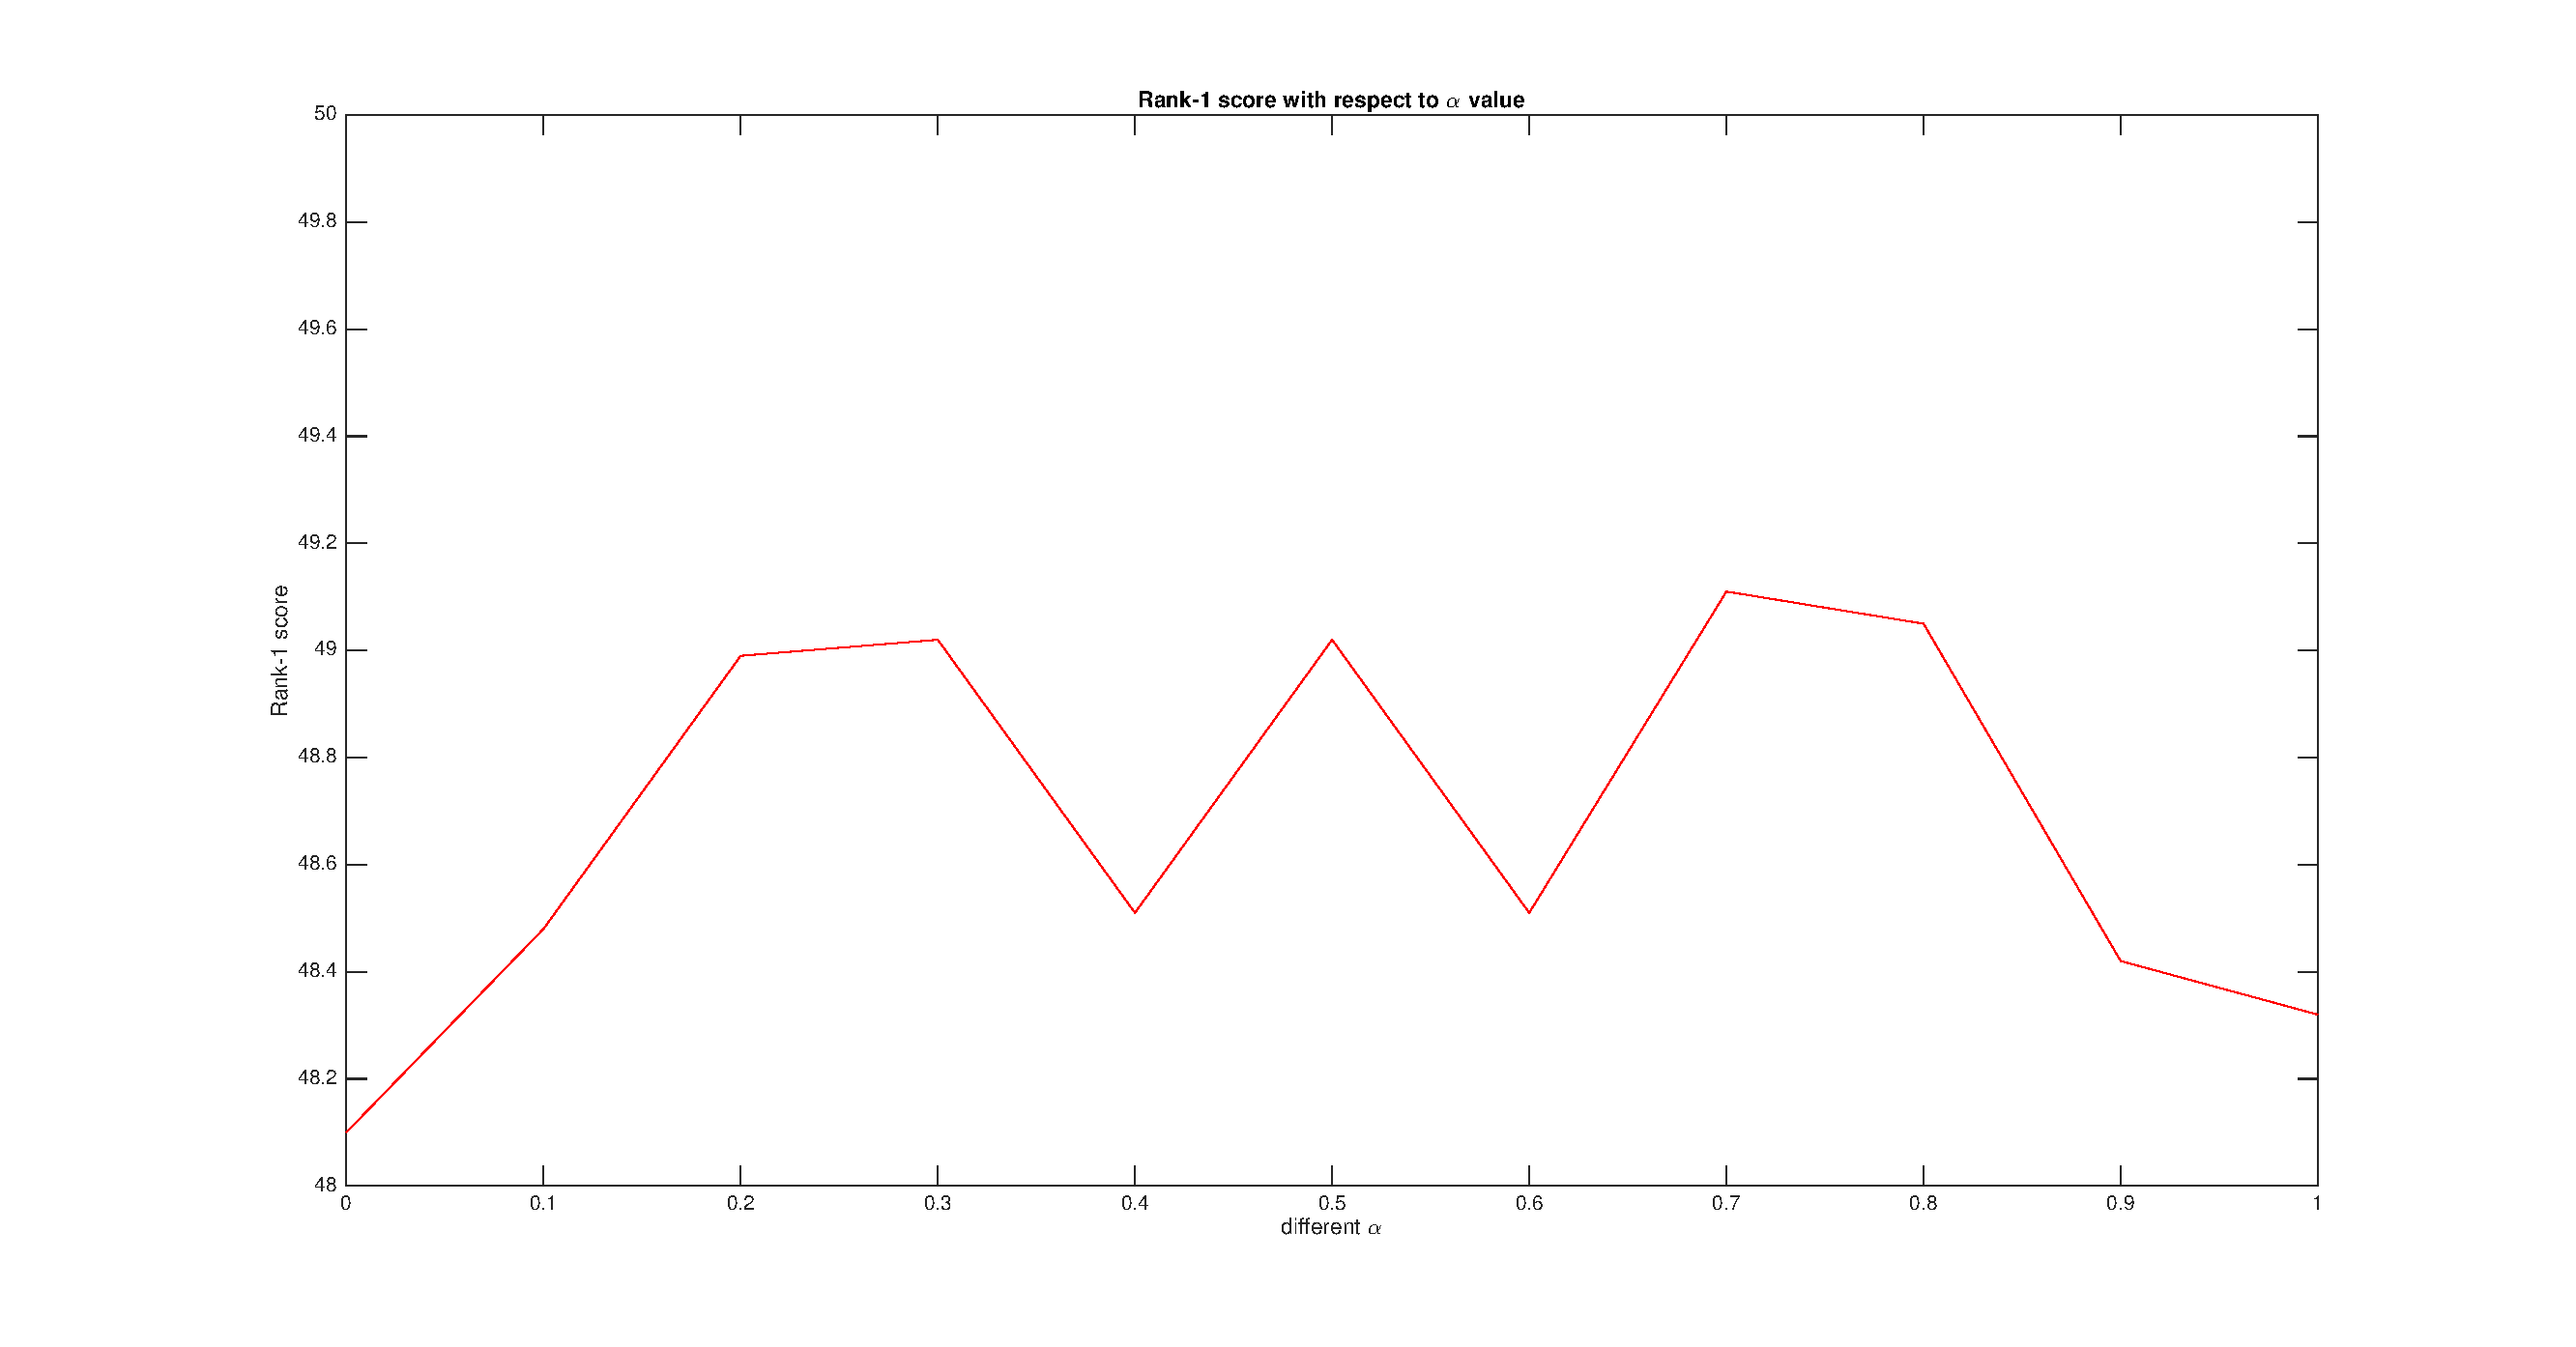
\includegraphics[width=1\linewidth]{Rank1scoresAlpha.eps}
%\vspace{-2em}
%\caption{Rank 1 scores with respect to $\alpha$ on VIPeR}
%\end{raggedleft}
%\end{figure}
%%-------------------------------------------------
%\begin{figure}
%\begin{raggedleft}
%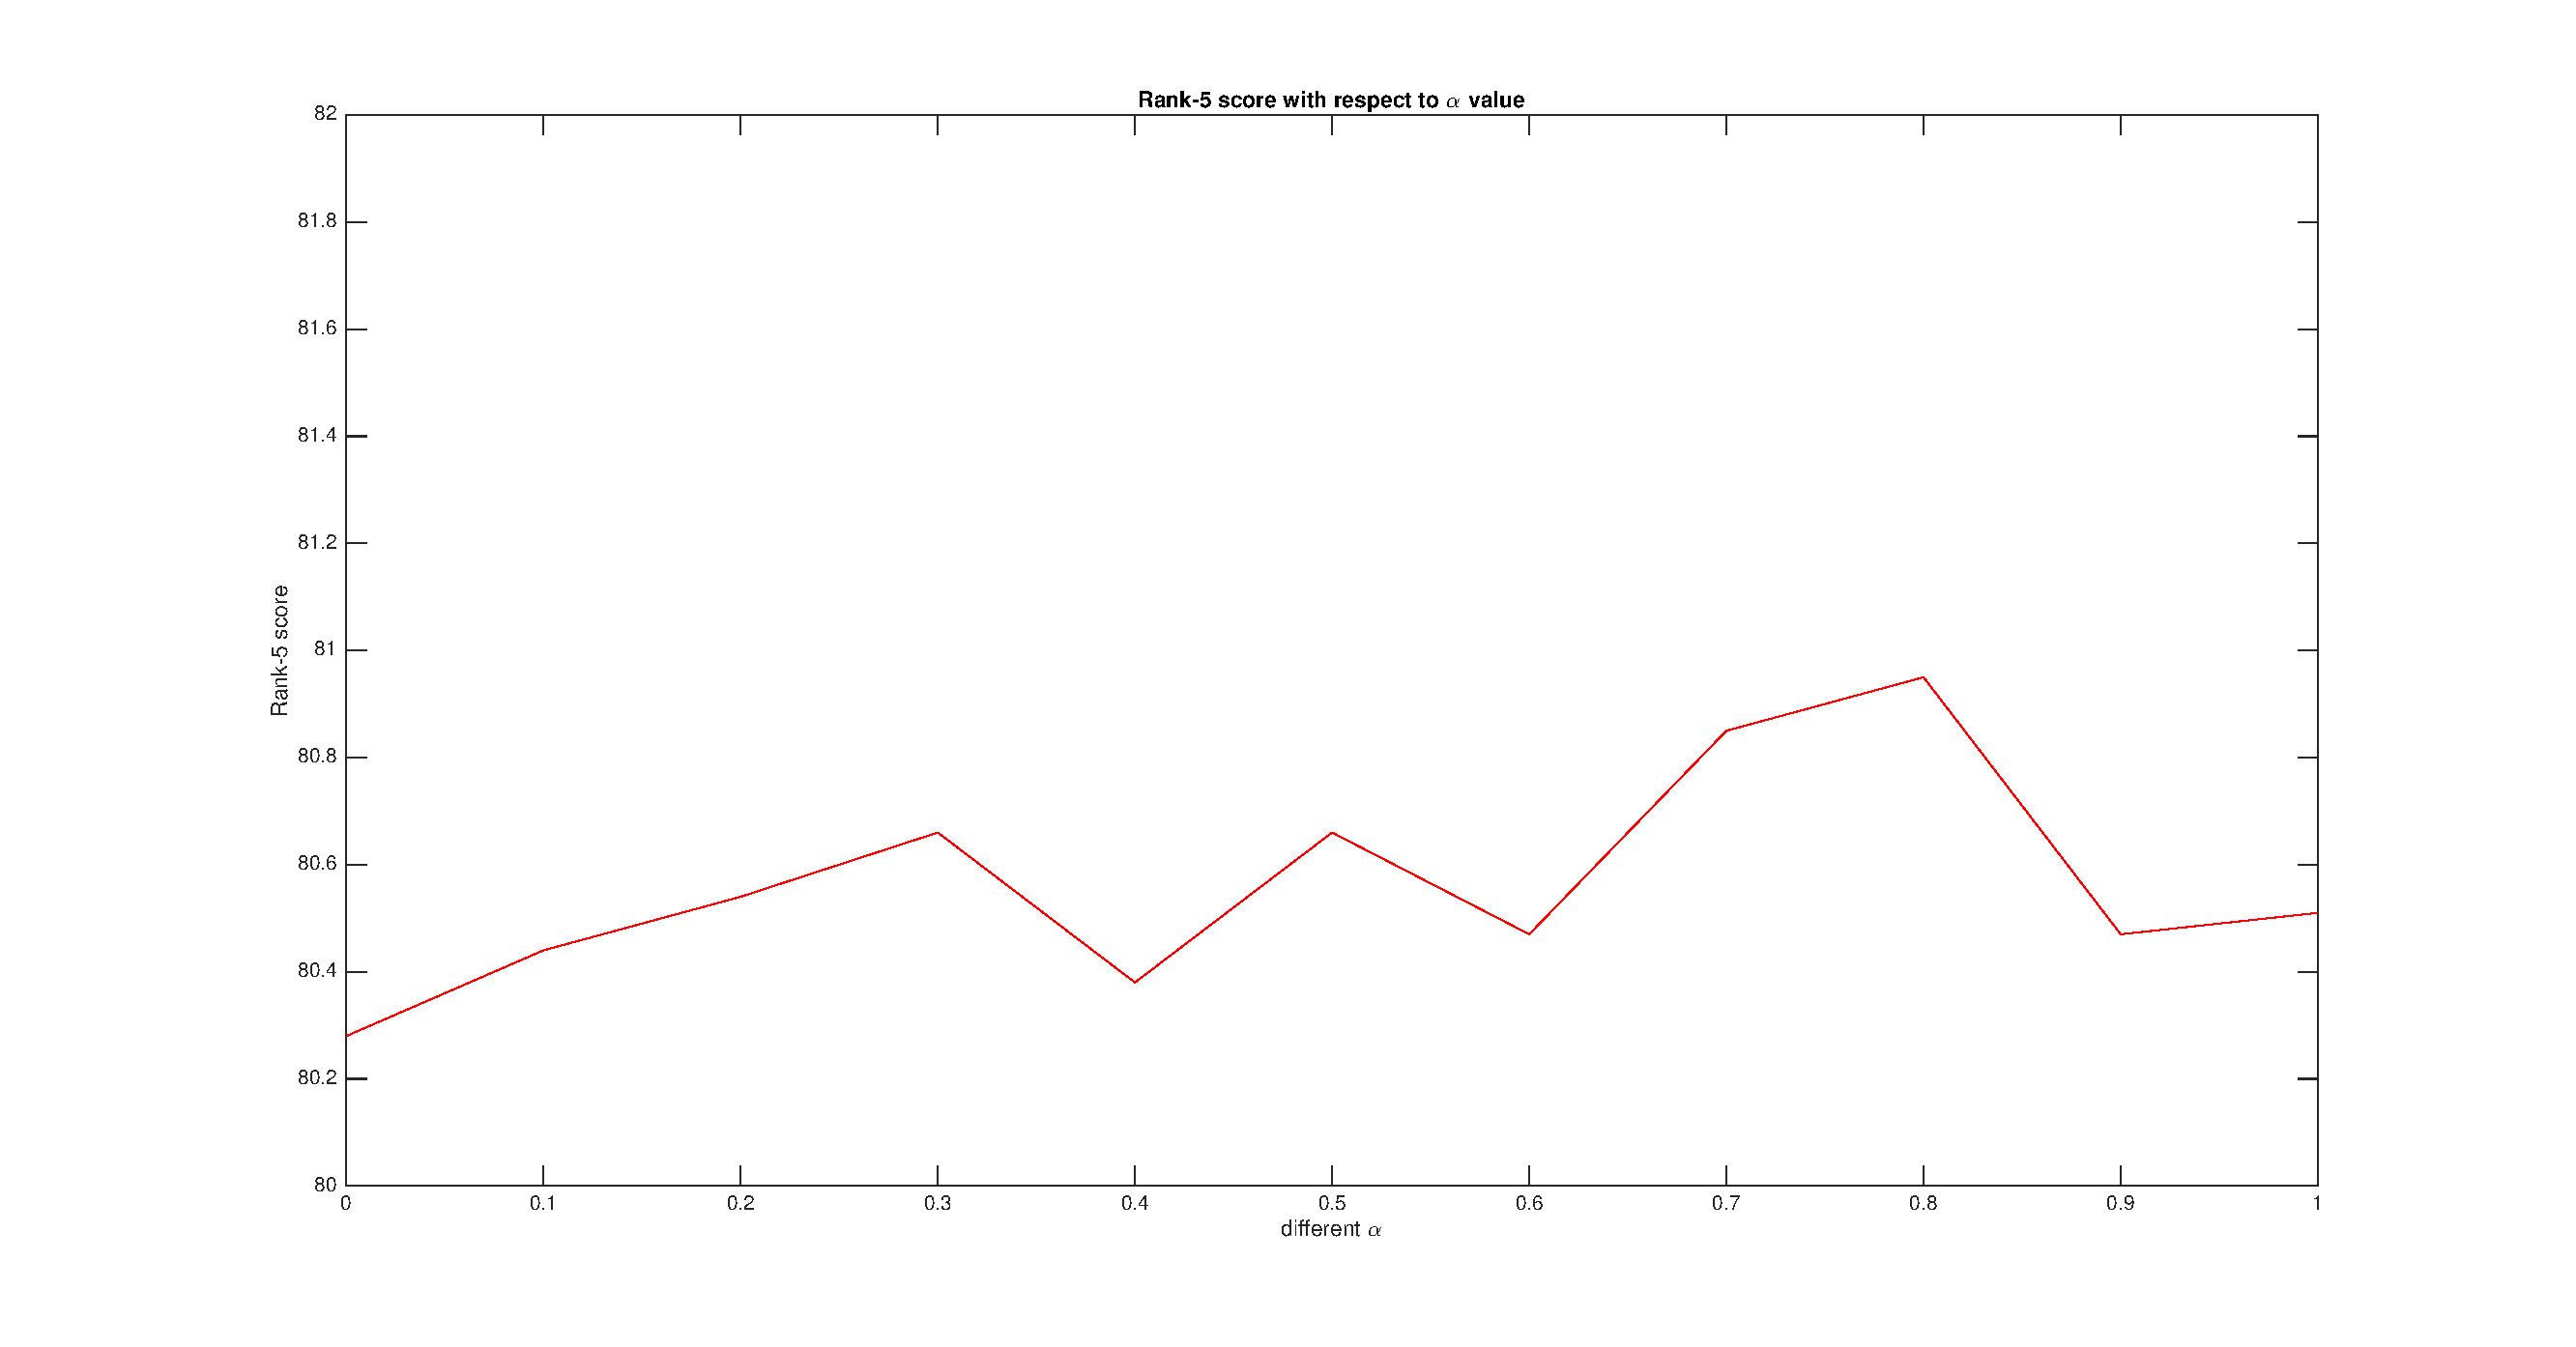
\includegraphics[width=1\linewidth]{Rank5scoresAlpha.eps}
%\vspace{-2em}
%\caption{Rank 5 scores with respect to $\alpha$ on VIPeR}
%\end{raggedleft}
%\end{figure}
%%-------------------------------------------------

%\textbf{Performance measuring} The cumulative matching curve is used to measure the descriptor performance. The score means the probability that the right match is within the top $n$ samples. A perfect CMC curve is expected to have a high rank-1 value and reaches 1 as fast as possible.
\subsection{Performance analysis}
In this paper, we compare proposed metric with other state-of-the-art metrics including NFST \cite{NFST}, XQDA \cite{LOMO}. NFST is a metric which learns a null space for descriptors so that the same class descriptors will be projected to a single point to minimize intraclass scatter matrix while different classes are projected to different points. This metric is a good solution to small sample problem in Re-ID. XQDA is similar with many other metrics, which learns a projection matrix $W$ and then a Mahalanobis SPD matrix $M$ is learned in the subspace. Those two metrics are proved to have state-of-the-art performance compared with many other methods. The GOG$_\text{rgb}$ in all tables means the hierarchical Gaussian descriptor in RGB color space while GOG$_\text{fusion}$ means the one in four different color spaces \{RGB, Lab, HSV, nRnG\}.\\
In \cite{GOG}, it has been shown that GOG + XQDA outperforms many other combinations, including Metric ensemble \cite{MetricEnsembles}, SCNCD \cite{SCNCD}, Semantic method \cite{SemanticMethod}, etc. In \cite{ NFST}, it has been shown LOMO + NFST outperforms metrics including LMNN \cite{LMNN}, KCCA \cite{KCCA}, ITML \cite{ITML}, KLFDA \cite{KLFDA}, MFA \cite{KernelVersionMetrics}, KISSME \cite{KISSME}, Similarity learning \cite{SimilarityLearning}, SCNCD \cite{SCNCD}, Mid-level filters \cite{MidlevelFilters} and Improved deep learning \cite{ImprovedCNN}. Based on the result that XQDA and NFST outperform other metrics, only XQDA and NFST are used in this thesis to compare with our proposed metric learning. 
\textbf{VIPeR} A comparison form is given in Table 3. Some of recent results are also included in this form. We can find that the rank scores are better than those of NFST and XQDA in terms of both GOG$_\text{rgb}$ and GOG$_\text{fusion}$. More specifically, the rank 1, rank 5, rank 10, rank 15 and rank 20 scores of proposed metric learning are 0.76\%, 0.92\%, 1.39\%, 1.08\%, 1.52\% higher than those of GOG$_\text{rgb}$ + XQDA. The rank 1, rank 5, rank 10, rank 15 and rank 20 GOG$_\text{fusion}$ scores of proposed metric learning are 0.35\%, -0.54\%, 0.98\%, 0.66\%, 0.79\% higher than GOG$_\text{fusion}$ + XQDA respectively. Also we can see that the proposed metric learning has a better performance than NFST. 
%-----------------------------------------------------------------------VIPeR
\begin{table}[H]\footnotesize
\caption{Performance of different metrics on VIPeR}
\centering
\begin{tabular}{|l|c|c|c|c|c|c|}
\hline
& \multicolumn{5}{|c|}{Rank(\%)} \\
\hline
Methods& 1 & 5 &10& 15&20\\
\hline
GOG$_\text{rgb}$+NFST& 43.23&73.16 &83.64 & 89.59&92.88\\  
\hline
GOG$_\text{rgb}$+XQDA& 43.01&73.92&83.86& 89.24& 92.37\\
\hline
%GOG$_\text{rgb}$+KLFDA&43.45 &74.68 &85.13 &90.54&93.70\\ 
%\hline
GOG$_\text{rgb}$+Proposed& \bftab 43.77 & \bftab 74.84 & \bftab 85.25 & \bftab 90.32 & \bftab 93.89\\   %43.48%, 74.59%, 85.35%, 90.47%, 93.67%
\hline
GOG$_\text{fusion}$+NFST&47.15& 76.39&87.31&91.74&94.49\\
\hline
GOG$_\text{fusion}$+XQDA& 47.97& \bftab 77.44 & 86.80& 91.27&93.70\\  
\hline
%GOG$_\text{fusion}$+KLFDA & 47.97&77.06& 87.56&91.80&94.18\\
%\hline
GOG$_\text{fusion}$+Proposed& \bftab 48.32&76.90& \bftab 87.78&\bftab91.93&\bftab94.49\\ %48.16%, 76.65%, 87.66%, 91.90%, 94.37% 
\hline
%--------------------------------------------------------------
\end{tabular}
\end{table}

\begin{figure}
\begin{raggedleft}
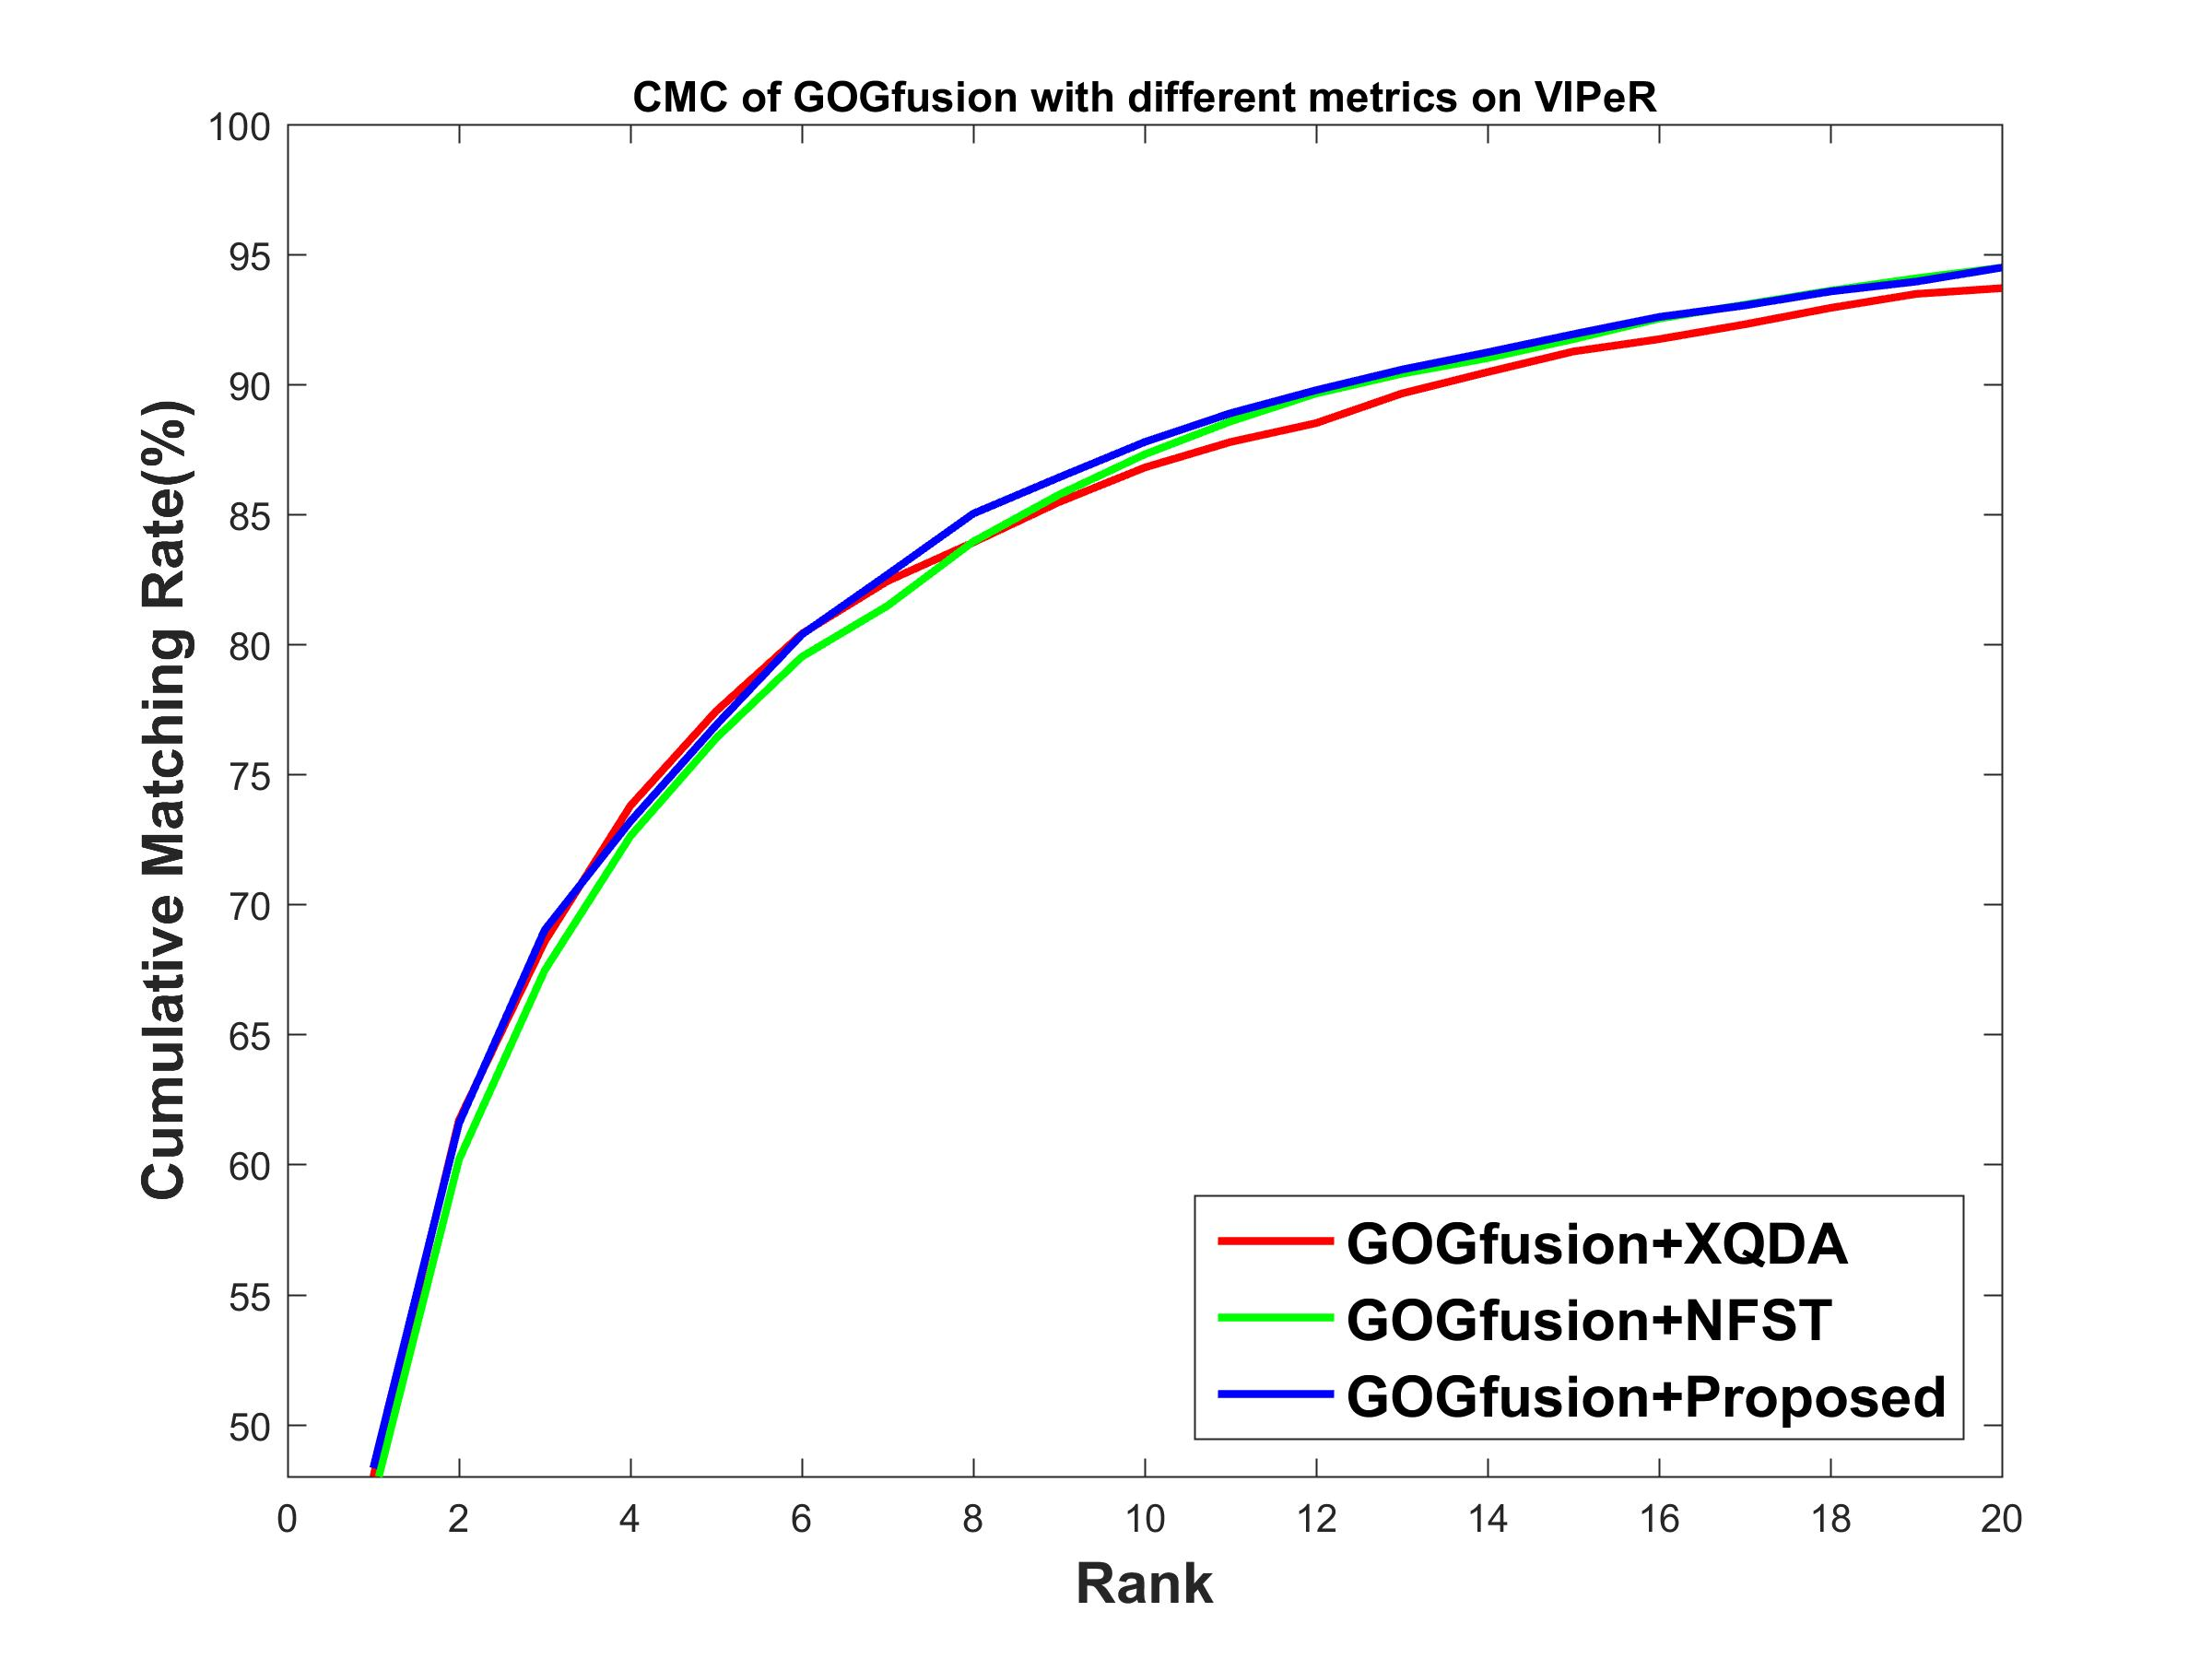
\includegraphics[width=1\linewidth]{VIPeR.jpg}
\vspace{-2em}
\caption{CMC curves on VIPeR comparing different metric learning}
\end{raggedleft}
\end{figure}

\textbf{CUHK1} We can find that the rank 1, rank5, rank 10, rank 15, rank 20 score of GOG$_\text{rgb}$ combined with proposed metric are 5.4\%, 4.18\%,3.31\%,2.16\%,1.46\% higher than XQDA, and 0.31\%, 1.22\%,1.34\%, 1.17\%, 1.11\% than NFST.  Also the  rank 1, rank5, rank 10, rank 15, rank 20 score of GOG$_\text{fusion}$ combined with proposed metric are 4.57\%, 2.64\%, 0.70\%, 1.33\%, 0.83\% higher than GOG$_\text{fusion}$ combined with XQDA, and 0.41\%, 0.83\%, 0.88\%, 1.09\%, 1.14\% than GOG$_\text{fusion}$ combined with NFST. 
%-------------------------------
%-----------------------------------------------------------------------CUHK1
\begin{table}\footnotesize
\caption{Performance of different metrics on CUHK1}
\centering
\begin{tabular}{|l|c|c|c|c|c|c|}
\hline
& \multicolumn{5}{|c|}{Rank(\%)} \\
\hline
Methods& 1 & 5 &10&15& 20\\
\hline
GOG$_\text{rgb}$+NFST&55.60 &83.02 &89.07 &91.98&93.56 \\ 
\hline
GOG$_\text{rgb}$+XQDA&50.51 &80.06 &87.10 &90.99&93.21 \\ 
\hline
%GOG$_\text{rgb}$+KLFDA&55.66&84.32&90.66&93.07& 94.63\\
%\hline
GOG$_\text{rgb}$+Proposed&\bftab55.91&\bftab84.24&\bftab90.41& \bftab93.15&\bftab94.67\\  %55.86%, 84.28%, 90.45%, 93.09%, 94.65% 
\hline
GOG$_\text{fusion}$+NFST&56.26 &83.66 &89.63 &92.22&93.70 \\ 
\hline
GOG$_\text{fusion}$+XQDA&52.10 &81.85&88.81 &91.98&94.01\\ 
\hline
%GOG$_\text{fusion}$+KLFDA & 56.60&84.67&90.41&93.13&94.81\\
%\hline
GOG$_\text{fusion}$+Proposed&\bftab56.67&\bftab84.49& \bftab90.51& \bftab93.31&\bftab94.84\\

\hline

\end{tabular}\newline
\end{table}
\begin{figure}
\begin{raggedleft}
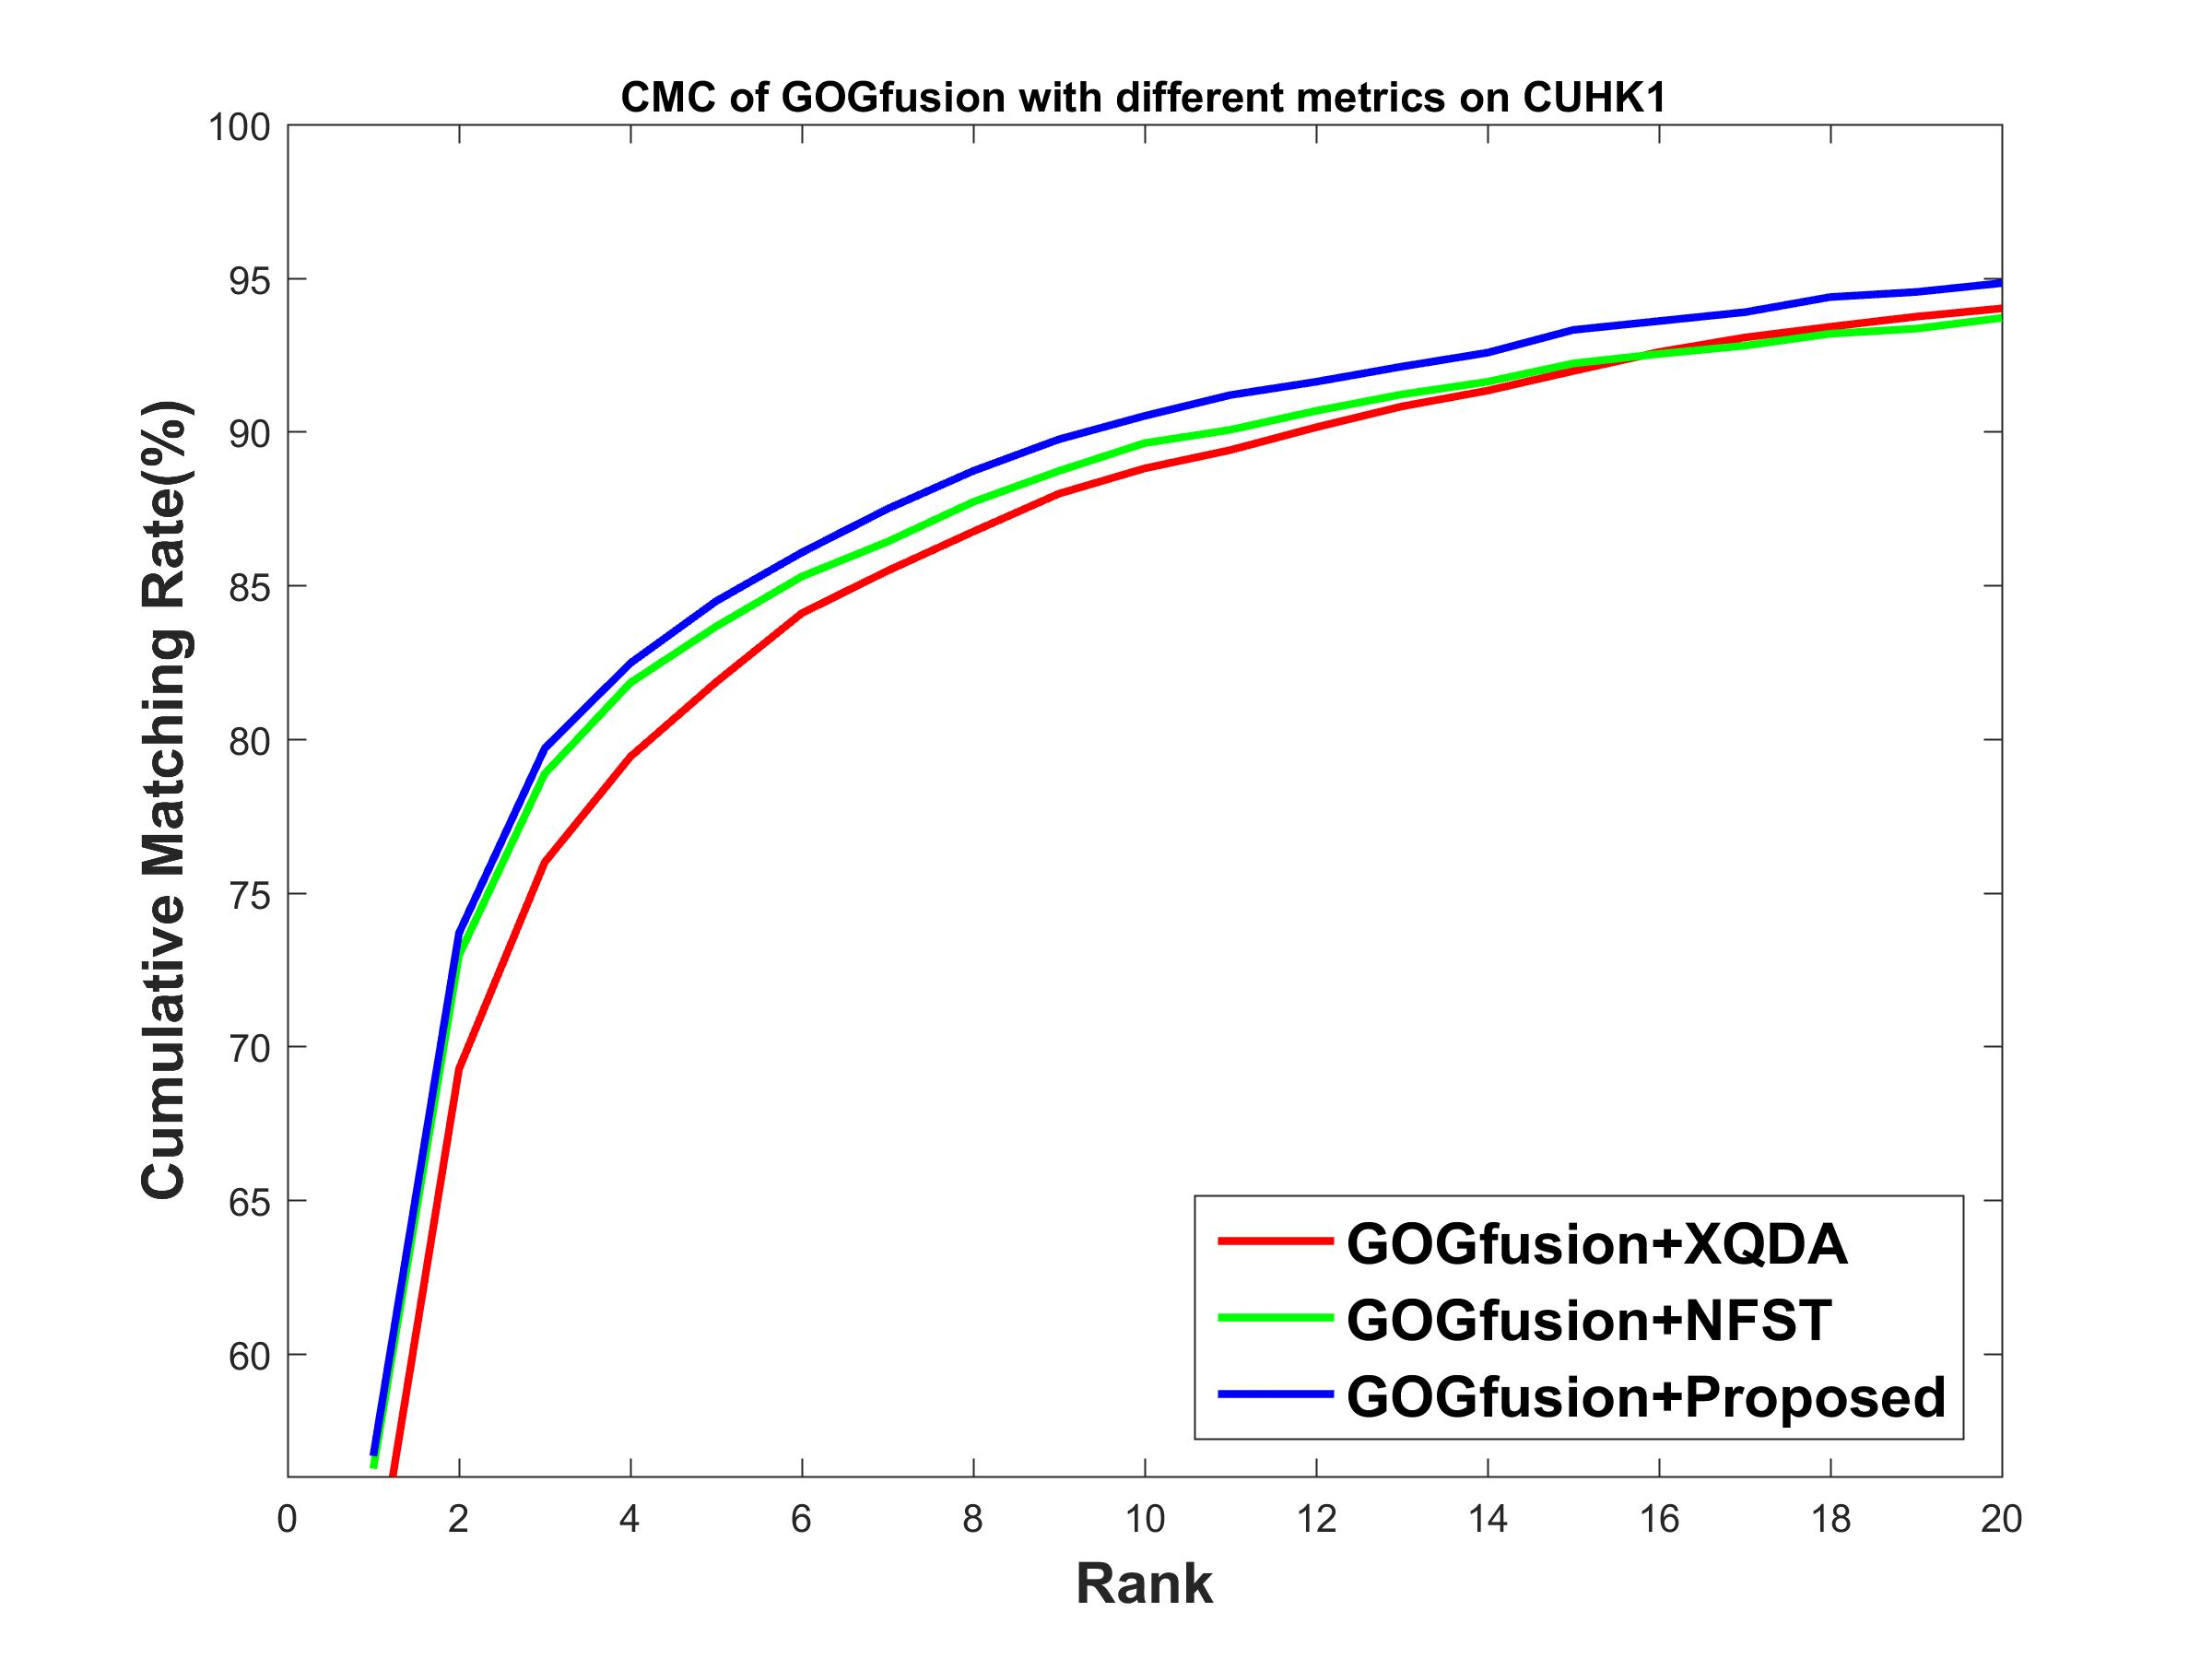
\includegraphics[width=1\linewidth]{CUHK1.jpg}
\vspace{-2em}
\caption{CMC curves on CUHK1 comparing different metric learning}
\end{raggedleft}
\end{figure}

%-----------------------------------------------------------------------PRID_2011

%\textbf{Prid\_2011}  The  rank 1, rank5, rank 10, rank 15, rank 20 score of GOG$_\text{fusion}$  combined with proposed metric are 6.1\%, 3.9\%, 4.5\%, 2.2\% and 1.3\% lower than GOG$_\text{fusion}$ combined with XQDA. The performance of NFST is slightly better than proposed metric. Also in terms of GOG$_\text{rgb}$ XQDA and NFST has better performance than the proposed one. So in this dataset the proposed metric has worse performance than XQDA and NFST.
%\begin{table}[H]
%\caption{Performance of different metrics on prid\_2011}
%\centering
%\begin{tabular}{|l|c|c|c|c|c|c|}
%\hline
%& \multicolumn{5}{|c|}{Rank(\%)} \\
%\hline
%Methods& 1 & 5 &10& 15&20\\
%\hline
%GOG$_\text{rgb}$+NFST&26.60 &53.80& 62.90&71.30&75.40 \\ 
%\hline
%GOG$_\text{rgb}$+XQDA&31.10 & 55.70& 66.10 & 72.40&76.10\\  
%\hline
%%GOG$_\text{rgb}$+KLFDA&23.70&51.70&63.10&69.90&73.60\\ 
%%\hline
%GOG$_\text{rgb}$+Proposed&23.80&52.20&63.50&70.20&73.50\\  %23.80%, 52.10%, 63.50%, 70.20%, 73.50%
%\hline
%GOG$_\text{fusion}$+NFST&34.10 &58.30& 67.60&73.80&78.30 \\  
%\hline
%GOG$_\text{fusion}$+XQDA&38.40& 61.30&70.80&75.60&79.30\\
%\hline
%%GOG$_\text{fusion}$+KLFDA & 31.90&56.90&66.60&72.60&77.50\\
%%\hline
%GOG$_\text{fusion}$+Proposed&32.30&57.40&66.30&73.40&78.00\\ %32.20%, 57.50%, 66.40%, 73.50%, 78.00(alpha = 0.7)   ()% 32.20%, 57.50%, 66.40%, 73.50%, 78.00%(alpha = 0.8)
%
%\hline
%
%\end{tabular}\newline
%\end{table}

%--------------------------------------
%\begin{figure}
%\begin{raggedleft}
%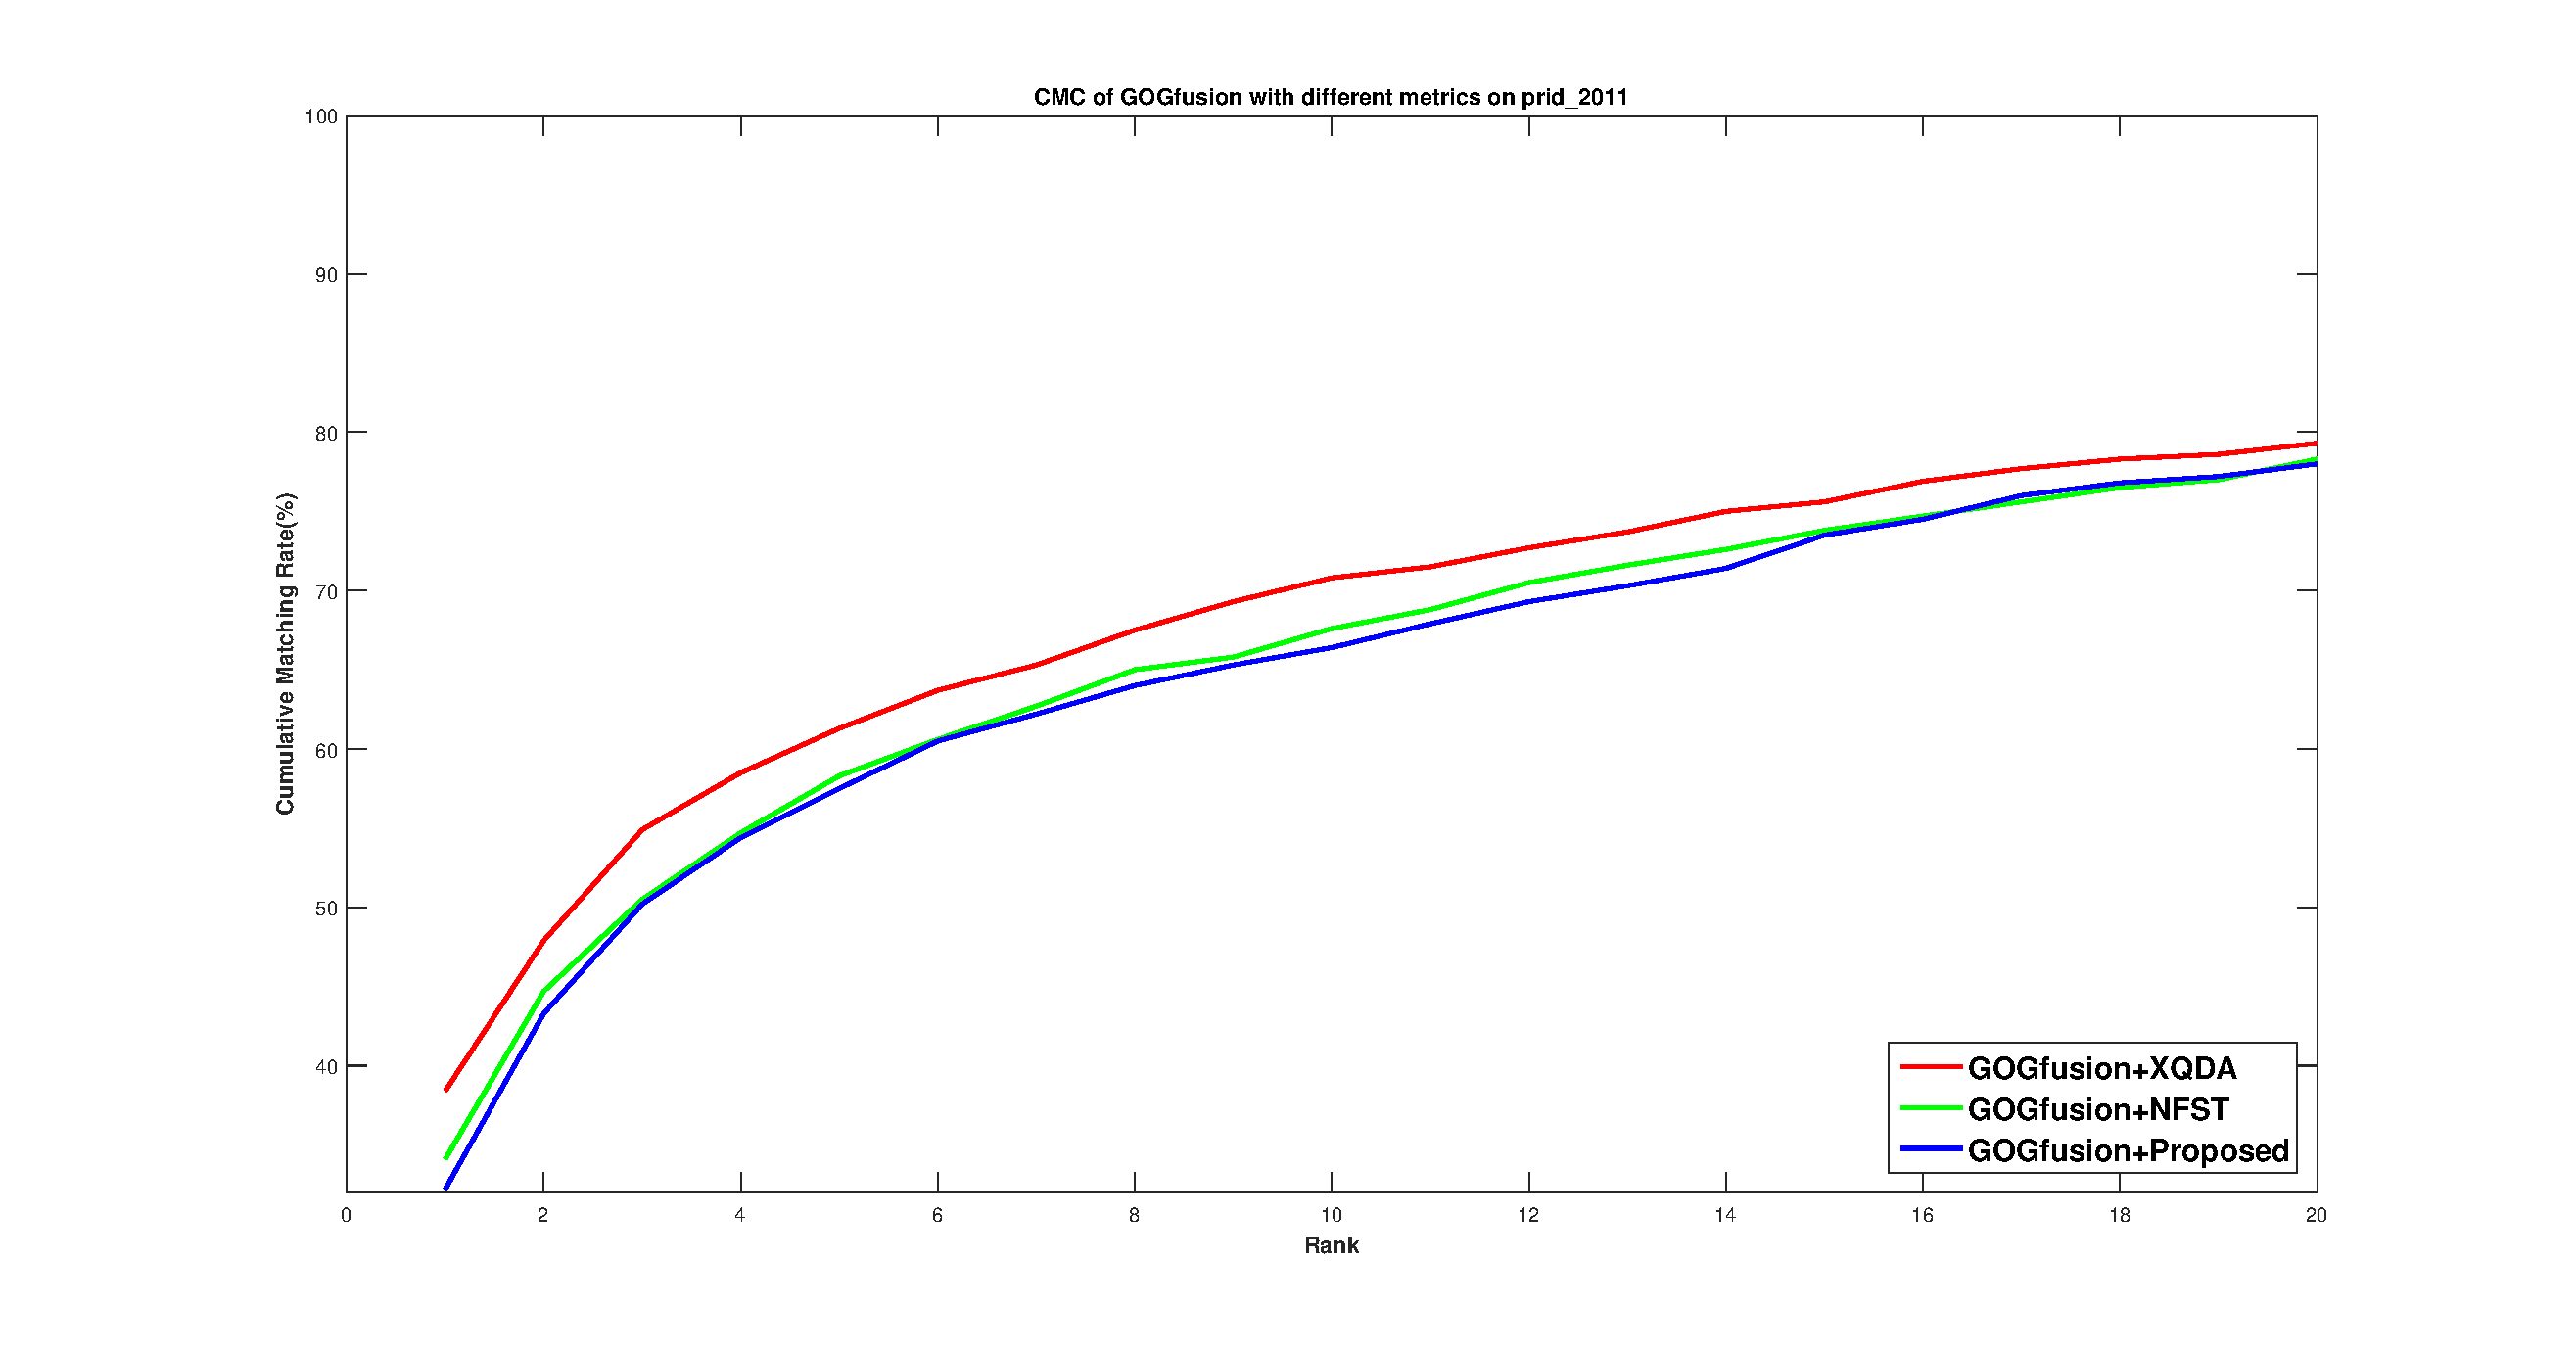
\includegraphics[width=1\linewidth]{prid2011.eps}
%\vspace{-2em}
%\caption{CMC curves on prid\_2011 comparing different metric learning}
%\end{raggedleft}
%\end{figure}

%-----------------------------------------------------------------------PRID_450S
\textbf{Prid\_450s} In this dataset, we can find the rank 1 score of XQDA and NFST is higher than proposed metric, but they have almost the same rank 5, rank 10, rank 15, and rank 20 scores with respect to both kinds of descriptors. 
\begin{table}\footnotesize
\caption{Performance of different metrics on prid\_450s}
\centering
\begin{tabular}{|l|c|c|c|c|c|c|}
\hline
& \multicolumn{5}{|c|}{Rank(\%)} \\
\hline
Methods& 1 & 5 &10& 15&20\\
\hline
GOG$_\text{rgb}$+NFST& 61.96&84.98 &90.53& 94.09&96.09 \\  %61.96%, 84.98%, 90.53%, 94.09%, 96.09%
\hline
GOG$_\text{rgb}$+XQDA&\bftab65.29 &\bftab85.02 & 91.13&\bftab94.76& \bftab96.49\\ 
\hline
%GOG$_\text{rgb}$+KLFDA&60.04&84.09&90.93&94.04&96.00 \\ 
%\hline
GOG$_\text{rgb}$+Proposed&60.71&84.53&\bftab91.29&94.13&96.27\\  %60.44%, 84.44%, 91.33%, 94.00%, 96.13%
\hline
GOG$_\text{fusion}$+NFST& 64.53&86.62 & 92.93&\bftab95.78&\bftab97.42 \\ 
\hline
GOG$_\text{fusion}$+XQDA&\bftab68.40 &\bftab 87.42&\bftab93.47 &95.69& 97.02\\ 
\hline
%GOG$_\text{fusion}$+KLFDA & 62.58&86.18&92.18&95.11&96.84\\
%\hline
GOG$_\text{fusion}$+Proposed&62.80&86.58&92.36&95.29& 96.89\\ % 62.62%, 86.44%, 92.36%, 95.20%, 96.93%(alpha = 0.7) 62.89%, 86.49%, 92.49%, 95.29%, 97.07%(alpha = 0.8)

\hline

\end{tabular}
\end{table}
%%--------------------------------------
\begin{figure}
\begin{raggedleft}
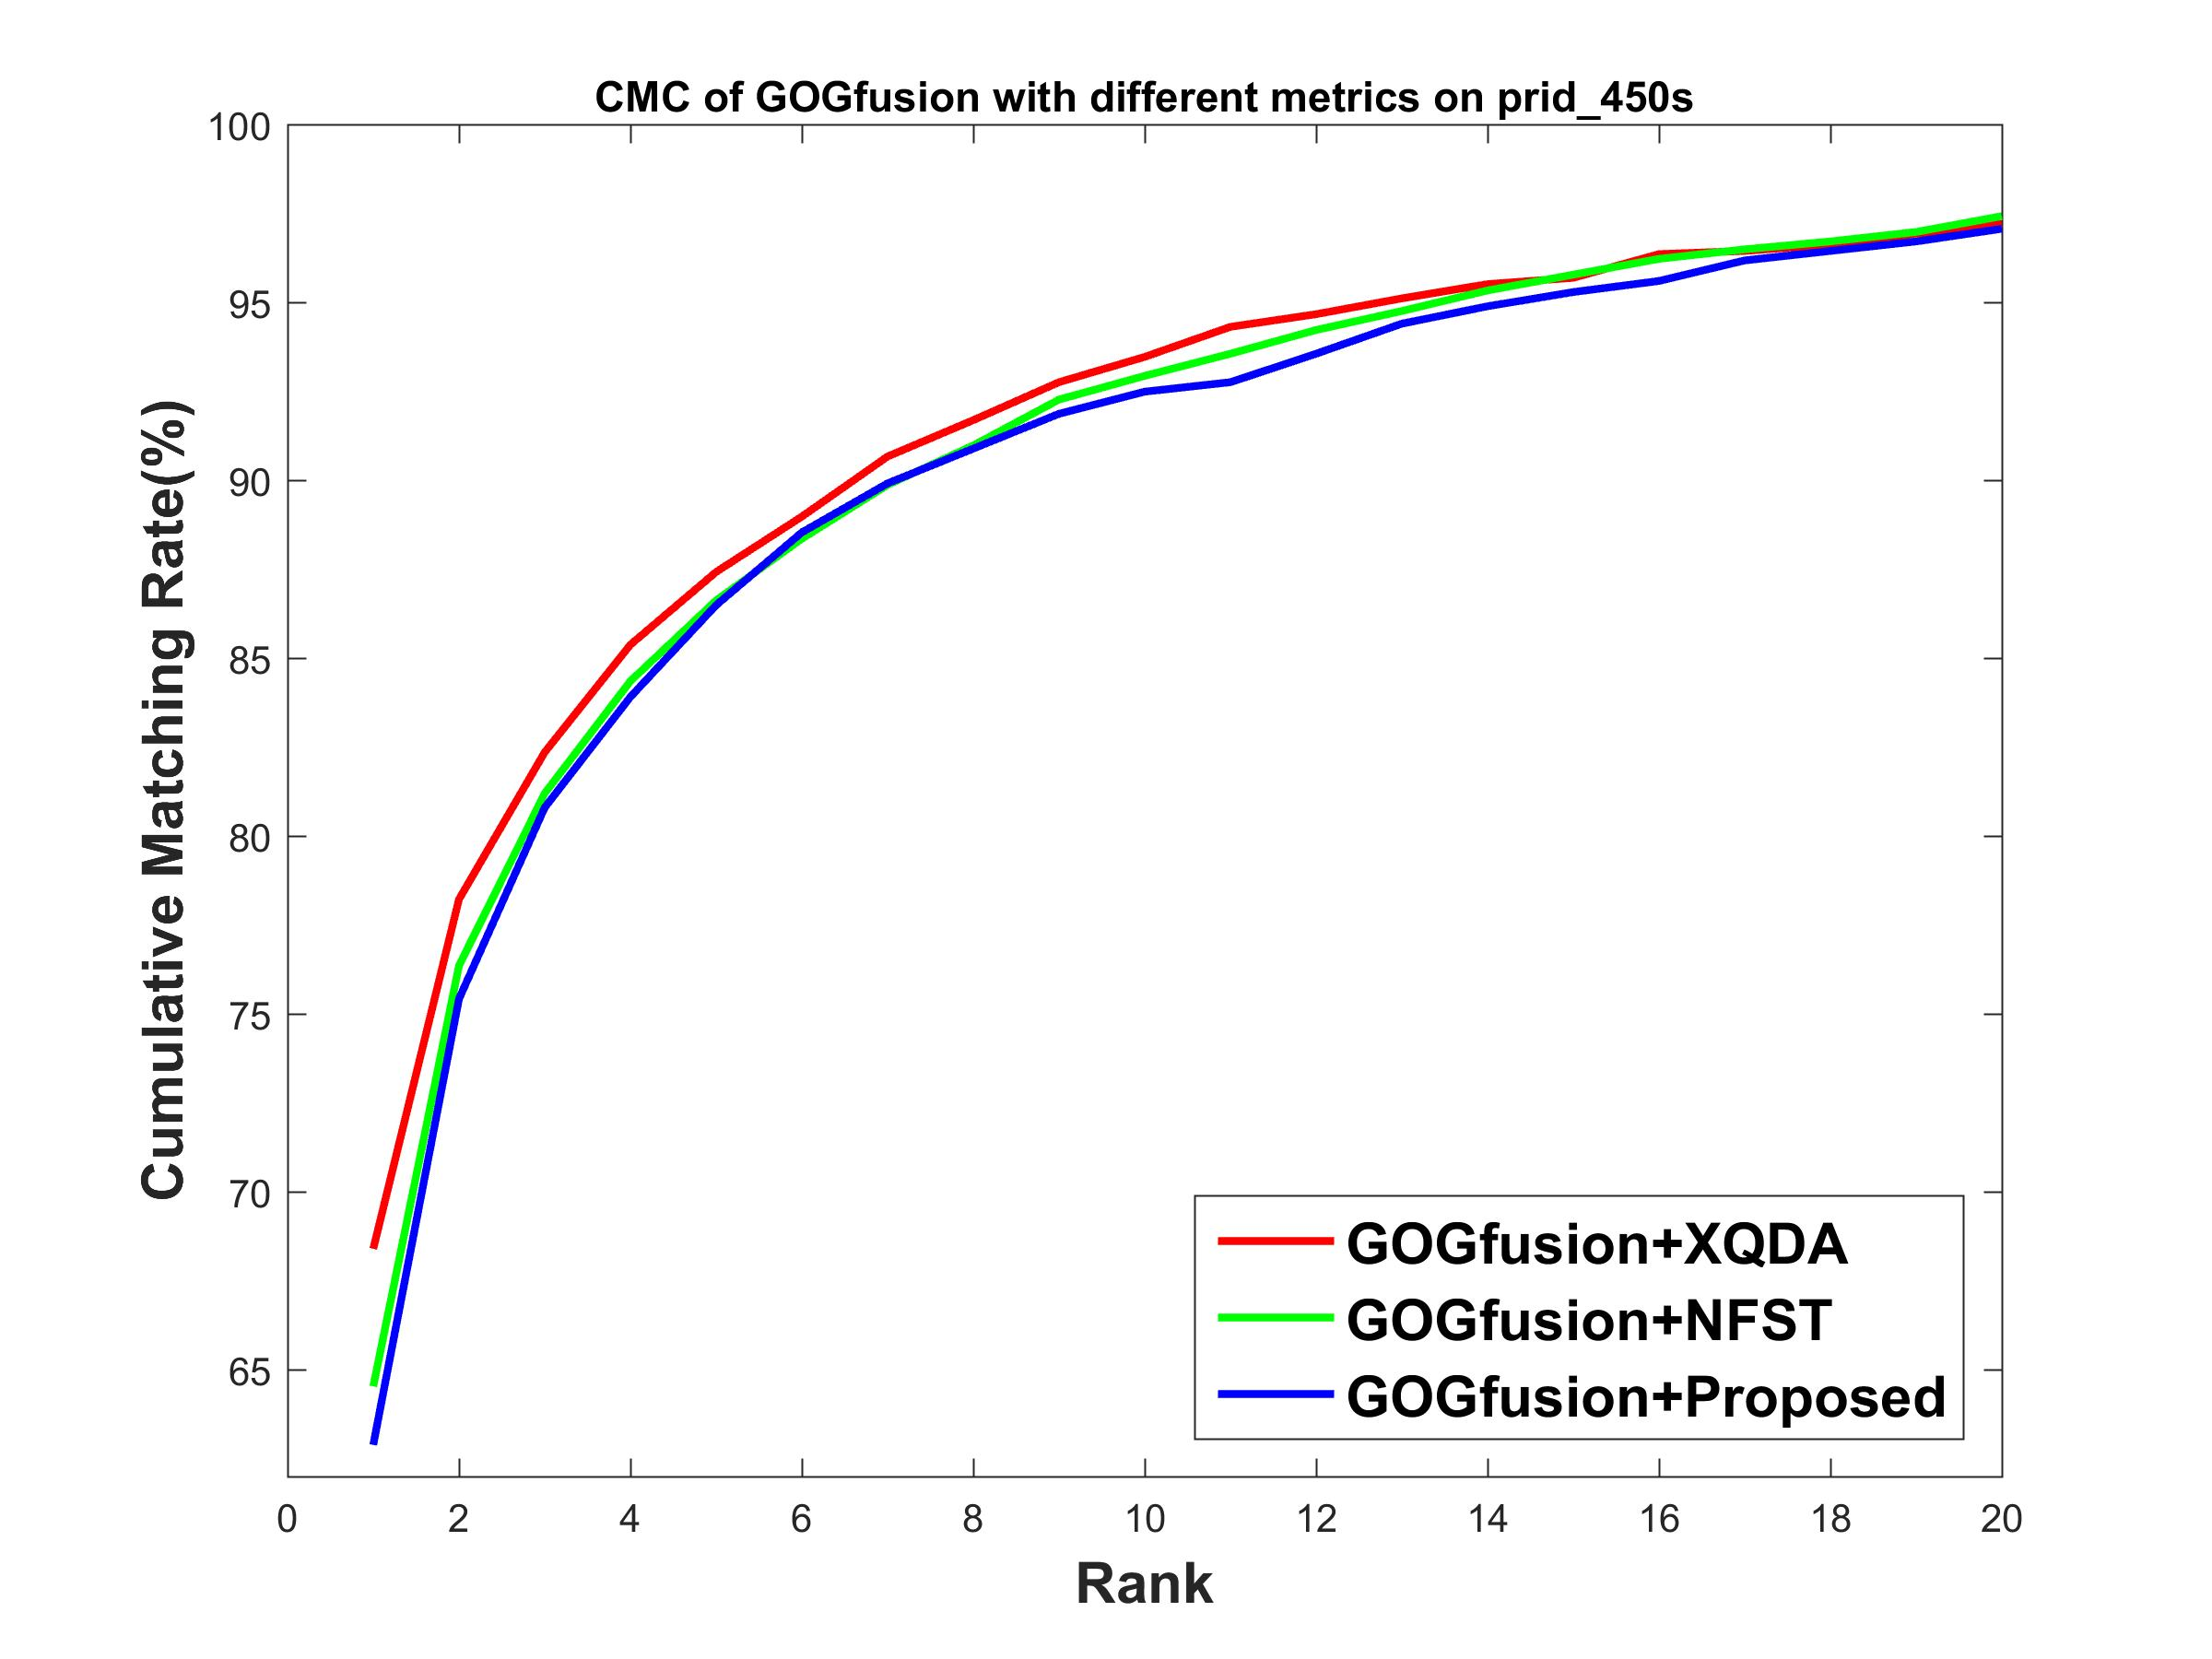
\includegraphics[width=1\linewidth]{prid_450s.jpg}
\vspace{-2em}
\caption{CMC curves on prid\_450s comparing different metric learning}
\end{raggedleft}
\end{figure}

%-----------------------------------------------------------------------GRID
%%--------------------------------------
\textbf{GRID} We can see that the rank 1 score of proposed metric are 0.24\% higher than XQDA and 0.88\% higher than NFST in terms of GOG$_\text{fusion}$, but XQDA outperforms proposed metric on rank 5, rank 10, rank 15 and rank 20 scores. Besides, proposed metric outperforms NFST on rank 5, rank 10, rank 15 scores.\\
\indent In summary, the Re-ID performance is improved in VIPeR, CUHK01 dataset, and has almost the same performance with NFST and XQDA on prid\_450s dataset. Specifically, proposed metric learning has the best rank 1 score in GRID dataset and its performance is only second to XQDA. The proposed metric has superior performance for following reasons: (1) dimension reduction by KLFDA exploits the nonlinearity and the loss of discriminant information between classes are minimized. (2) the simplified relative distance limitation optimization helps to confine the Mahalanobis distance matrix $\bm{M}$ to discriminate different classes.  
%------------------------------------------------------------------------
\begin{table}\footnotesize
\caption{Performance of different metrics on GRID}
\centering
\begin{tabular}{|l|c|c|c|c|c|c|}
\hline
& \multicolumn{5}{|c|}{Rank(\%)} \\
\hline
Methods& 1 & 5 &10& 15&20\\
\hline
GOG$_\text{rgb}$+NFST& 21.84&41.28 &50.96& 57.44&62.88 \\ 
\hline
GOG$_\text{rgb}$+XQDA& \bftab22.64&\bftab43.92 &\bftab55.12 &\bftab61.12&\bftab66.56\\ 
\hline
%GOG$_\text{rgb}$+KLFDA&23.44&43.04&52.16&59.12&64.88 \\ 
%\hline
GOG$_\text{rgb}$+Proposed&\bftab22.64&43.68&52.00&59.04&65.04\\  %22.80%, 43.76%, 52.08%, 59.04%, 65.12%
\hline
GOG$_\text{fusion}$+NFST& 23.04&44.40 &54.40 &61.84&66.56\\ 
\hline
GOG$_\text{fusion}$+XQDA& 23.68&\bftab47.28 &\bftab58.40 &\bftab65.84&\bftab69.68 \\ 
\hline
%GOG$_\text{fusion}$+KLFDA &23.76&44.40& 55.36&61.76& 66.48\\
%\hline
GOG$_\text{fusion}$+Proposed&\bftab23.92&44.64&54.88&62.32&66.40\\ %23.84%, 44.64%, 55.04%, 62.24%, 66.24%
\hline

\end{tabular}
\end{table}
%--------------------------------------
\begin{figure}
\begin{raggedleft}
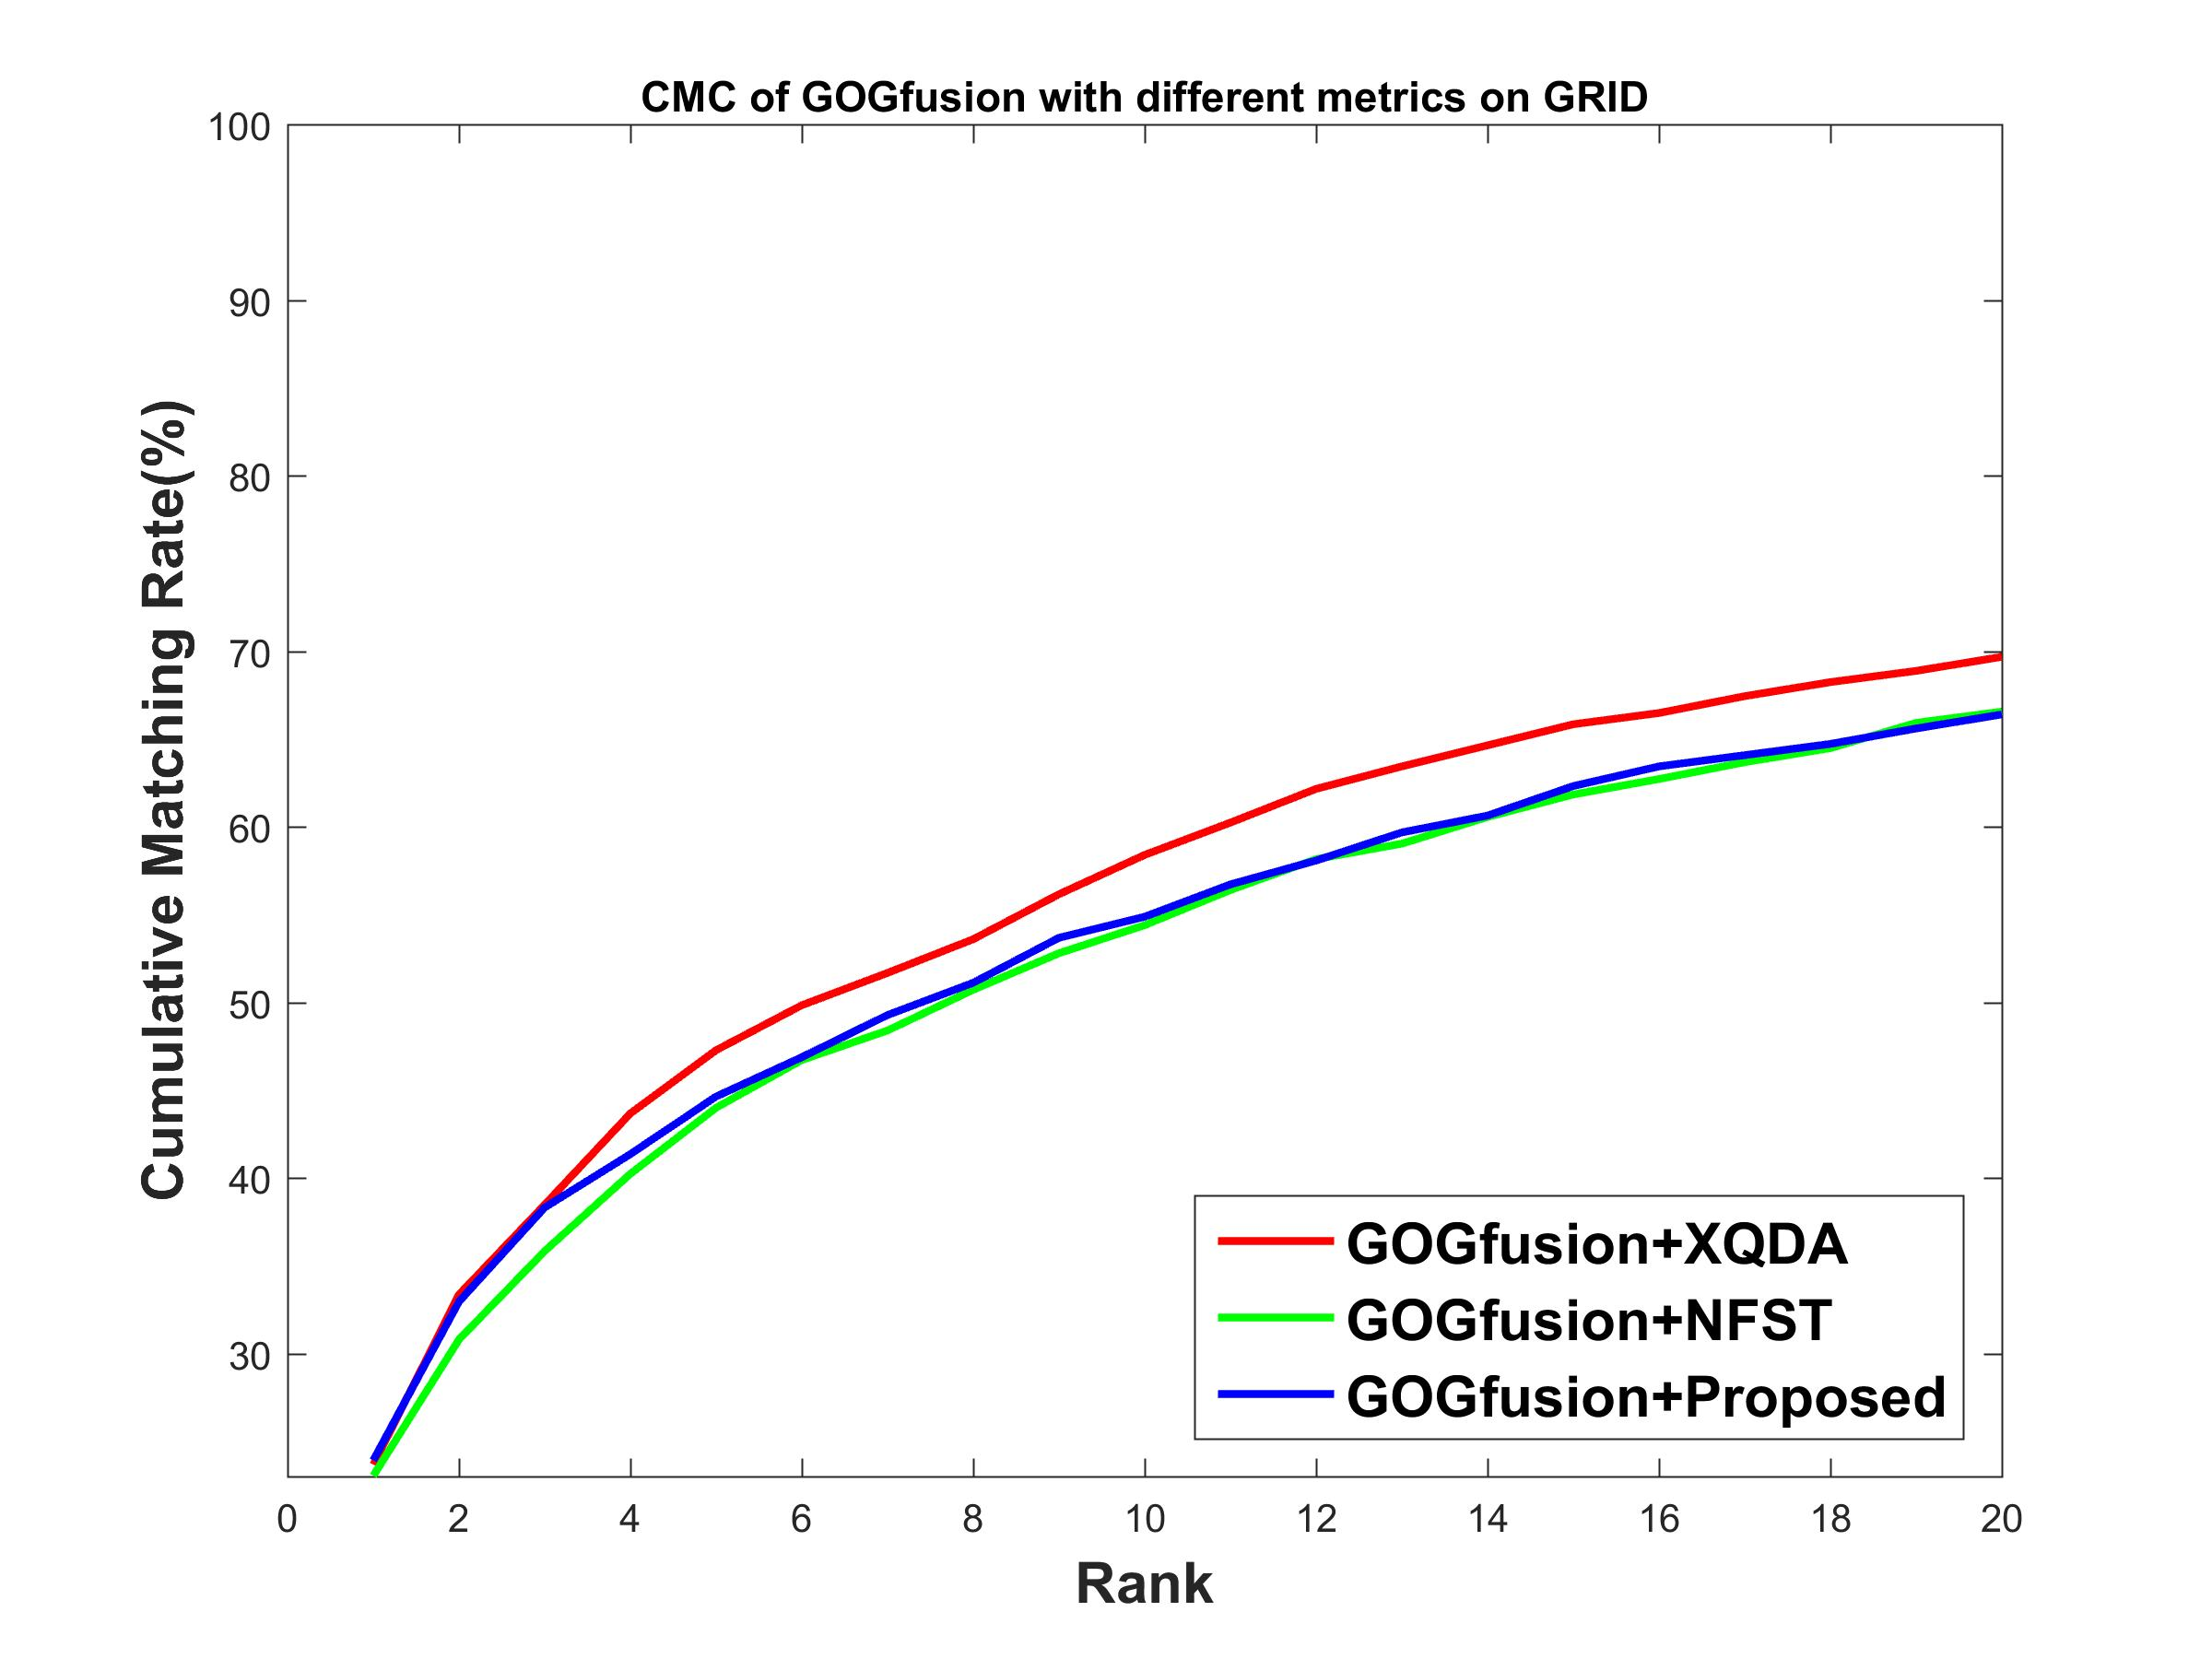
\includegraphics[width=1\linewidth]{GRID.jpg}
\vspace{-2em}
\caption{CMC curves on GRID comparing different metric learning}
\end{raggedleft}
\end{figure}

\subsection{Time cost}
The training time increases when the dataset size increases. For the CUHK1 dataset which has most training pairs, it takes half an hour to train the metric on a desktop PC with a 16GB RAM, Intel i5 processor. For datasets with fewer training pairs like Prid\_2011 and GRID, it takes no more than five minutes.
\section{Conclusion}
In this paper we combined KLFDA with gradient descent method based metric learning. An SPD matrix is learned on the lower dimension space after dimensionality reduction by KLFDA. By comparison and analysis we can find the proposed metric has better performance than NFST and XQDA on VIPeR and CUHK1 datasets, but XQDA and NFST outperforms the proposed metric learning on Prid\_2011 and Prid\_450s. On GRID dataset the proposed metric learning has better rank 1 score than NFST and its performance is only second to XQDA.\\
\indent In summary, our proposed metric improved the Re-ID accuracy in VIPeR and CUHK1 datasets, and has almost the same performance with NFST and XQDA in the prid\_450s dataset. Furthermore, the proposed metric learning has the best rank 1 score in the GRID dataset and its performance is only second to XQDA. The proposed metric has superior performance for the following reasons: (1) dimension reduction by KLFDA exploits the nonlinearity, and the loss of discriminant information between classes is minimized; (2) the simplified relative distance limitation optimization helps to confine the Mahalanobis distance matrix $\bm{M}$ to discriminate different classes.




%%----------------------------------------------------------------------------------------------------------------------------------------------------------------------------------------------------
%%----------------------------------------------------------------------------------------------------------------------------------------------------------------------------------------------------
%\subsection{Language}
%
%All manuscripts must be in English.
%
%\subsection{Dual submission}
%
%Please refer to the author guidelines on the ICCV 2017 web page for a
%discussion of the policy on dual submissions.
%
%\subsection{Paper length}
%For ICCV 2017, the rules about paper length have changed, so please read this section carefully. Papers, excluding the references section, must be no longer than eight pages in length. There are no page limits for references.
%
%Overlength papers will simply not be reviewed.  This includes papers
%where the margins and formatting are deemed to have been significantly
%altered from those laid down by this style guide.  Note that this
%\LaTeX\ guide already sets figure captions and references in a smaller font.
%The reason such papers will not be reviewed is that there is no provision for
%supervised revisions of manuscripts.  The reviewing process cannot determine
%the suitability of the paper for presentation in eight pages if it is
%reviewed in eleven.  
%
%%-------------------------------------------------------------------------
%\subsection{The ruler}
%The \LaTeX\ style defines a printed ruler which should be present in the
%version submitted for review.  The ruler is provided in order that
%reviewers may comment on particular lines in the paper without
%circumlocution.  If you are preparing a document using a non-\LaTeX\
%document preparation system, please arrange for an equivalent ruler to
%appear on the final output pages.  The presence or absence of the ruler
%should not change the appearance of any other content on the page.  The
%camera ready copy should not contain a ruler. (\LaTeX\ users may uncomment
%the \verb'\iccvfinalcopy' command in the document preamble.)  Reviewers:
%note that the ruler measurements do not align well with lines in the paper
%--- this turns out to be very difficult to do well when the paper contains
%many figures and equations, and, when done, looks ugly.  Just use fractional
%references (e.g.\ this line is $095.5$), although in most cases one would
%expect that the approximate location will be adequate.
%
%\subsection{Mathematics}
%
%Please number all of your sections and displayed equations.  It is
%important for readers to be able to refer to any particular equation.  Just
%because you didn't refer to it in the text doesn't mean some future reader
%might not need to refer to it.  It is cumbersome to have to use
%circumlocutions like ``the equation second from the top of page 3 column
%1''.  (Note that the ruler will not be present in the final copy, so is not
%an alternative to equation numbers).  All authors will benefit from reading
%Mermin's description of how to write mathematics:
%\url{http://www.pamitc.org/documents/mermin.pdf}.
%
%
%\subsection{Blind review}
%
%Many authors misunderstand the concept of anonymizing for blind
%review.  Blind review does not mean that one must remove
%citations to one's own work---in fact it is often impossible to
%review a paper unless the previous citations are known and
%available.
%
%Blind review means that you do not use the words ``my'' or ``our''
%when citing previous work.  That is all.  (But see below for
%techreports.)
%
%Saying ``this builds on the work of Lucy Smith [1]'' does not say
%that you are Lucy Smith; it says that you are building on her
%work.  If you are Smith and Jones, do not say ``as we show in
%[7]'', say ``as Smith and Jones show in [7]'' and at the end of the
%paper, include reference 7 as you would any other cited work.
%
%An example of a bad paper just asking to be rejected:
%\begin{quote}
%\begin{center}
%    An analysis of the frobnicatable foo filter.
%\end{center}
%
%   In this paper we present a performance analysis of our
%   previous paper [1], and show it to be inferior to all
%   previously known methods.  Why the previous paper was
%   accepted without this analysis is beyond me.
%
%   [1] Removed for blind review
%\end{quote}
%
%
%An example of an acceptable paper:
%
%\begin{quote}
%\begin{center}
%     An analysis of the frobnicatable foo filter.
%\end{center}
%
%   In this paper we present a performance analysis of the
%   paper of Smith \etal [1], and show it to be inferior to
%   all previously known methods.  Why the previous paper
%   was accepted without this analysis is beyond me.
%
%   [1] Smith, L and Jones, C. ``The frobnicatable foo
%   filter, a fundamental contribution to human knowledge''.
%   Nature 381(12), 1-213.
%\end{quote}
%
%If you are making a submission to another conference at the same time,
%which covers similar or overlapping material, you may need to refer to that
%submission in order to explain the differences, just as you would if you
%had previously published related work.  In such cases, include the
%anonymized parallel submission~\cite{Authors14} as additional material and
%cite it as
%\begin{quote}
%[1] Authors. ``The frobnicatable foo filter'', F\&G 2014 Submission ID 324,
%Supplied as additional material {\tt fg324.pdf}.
%\end{quote}
%
%Finally, you may feel you need to tell the reader that more details can be
%found elsewhere, and refer them to a technical report.  For conference
%submissions, the paper must stand on its own, and not {\em require} the
%reviewer to go to a techreport for further details.  Thus, you may say in
%the body of the paper ``further details may be found
%in~\cite{Authors14b}''.  Then submit the techreport as additional material.
%Again, you may not assume the reviewers will read this material.
%
%Sometimes your paper is about a problem which you tested using a tool which
%is widely known to be restricted to a single institution.  For example,
%let's say it's 1969, you have solved a key problem on the Apollo lander,
%and you believe that the ICCV70 audience would like to hear about your
%solution.  The work is a development of your celebrated 1968 paper entitled
%``Zero-g frobnication: How being the only people in the world with access to
%the Apollo lander source code makes us a wow at parties'', by Zeus \etal.
%
%You can handle this paper like any other.  Don't write ``We show how to
%improve our previous work [Anonymous, 1968].  This time we tested the
%algorithm on a lunar lander [name of lander removed for blind review]''.
%That would be silly, and would immediately identify the authors. Instead
%write the following:
%\begin{quotation}
%\noindent
%   We describe a system for zero-g frobnication.  This
%   system is new because it handles the following cases:
%   A, B.  Previous systems [Zeus et al. 1968] didn't
%   handle case B properly.  Ours handles it by including
%   a foo term in the bar integral.
%
%   ...
%
%   The proposed system was integrated with the Apollo
%   lunar lander, and went all the way to the moon, don't
%   you know.  It displayed the following behaviours
%   which show how well we solved cases A and B: ...
%\end{quotation}
%As you can see, the above text follows standard scientific convention,
%reads better than the first version, and does not explicitly name you as
%the authors.  A reviewer might think it likely that the new paper was
%written by Zeus \etal, but cannot make any decision based on that guess.
%He or she would have to be sure that no other authors could have been
%contracted to solve problem B.
%
%FAQ: Are acknowledgements OK?  No.  Leave them for the final copy.
%
%
%\begin{figure}[t]
%\begin{center}
%\fbox{\rule{0pt}{2in} \rule{0.9\linewidth}{0pt}}
%   %\includegraphics[width=0.8\linewidth]{egfigure.eps}
%\end{center}
%   \caption{Example of caption.  It is set in Roman so that mathematics
%   (always set in Roman: $B \sin A = A \sin B$) may be included without an
%   ugly clash.}
%\label{fig:long}
%\label{fig:onecol}
%\end{figure}
%
%\subsection{Miscellaneous}
%
%\noindent
%Compare the following:\\
%\begin{tabular}{ll}
% \verb'$conf_a$' &  $conf_a$ \\
% \verb'$\mathit{conf}_a$' & $\mathit{conf}_a$
%\end{tabular}\\
%See The \TeX book, p165.
%
%The space after \eg, meaning ``for example'', should not be a
%sentence-ending space. So \eg is correct, {\em e.g.} is not.  The provided
%\verb'\eg' macro takes care of this.
%
%When citing a multi-author paper, you may save space by using ``et alia'',
%shortened to ``\etal'' (not ``{\em et.\ al.}'' as ``{\em et}'' is a complete word.)
%However, use it only when there are three or more authors.  Thus, the
%following is correct: ``
%   Frobnication has been trendy lately.
%   It was introduced by Alpher~\cite{Alpher02}, and subsequently developed by
%   Alpher and Fotheringham-Smythe~\cite{Alpher03}, and Alpher \etal~\cite{Alpher04}.''
%
%This is incorrect: ``... subsequently developed by Alpher \etal~\cite{Alpher03} ...''
%because reference~\cite{Alpher03} has just two authors.  If you use the
%\verb'\etal' macro provided, then you need not worry about double periods
%when used at the end of a sentence as in Alpher \etal.
%
%For this citation style, keep multiple citations in numerical (not
%chronological) order, so prefer \cite{Alpher03,Alpher02,Authors14} to
%\cite{Alpher02,Alpher03,Authors14}.
%
%
%\begin{figure*}
%\begin{center}
%\fbox{\rule{0pt}{2in} \rule{.9\linewidth}{0pt}}
%\end{center}
%   \caption{Example of a short caption, which should be centered.}
%\label{fig:short}
%\end{figure*}
%
%%------------------------------------------------------------------------
%\section{Formatting your paper}
%
%All text must be in a two-column format. The total allowable width of the
%text area is $6\frac78$ inches (17.5 cm) wide by $8\frac78$ inches (22.54
%cm) high. Columns are to be $3\frac14$ inches (8.25 cm) wide, with a
%$\frac{5}{16}$ inch (0.8 cm) space between them. The main title (on the
%first page) should begin 1.0 inch (2.54 cm) from the top edge of the
%page. The second and following pages should begin 1.0 inch (2.54 cm) from
%the top edge. On all pages, the bottom margin should be 1-1/8 inches (2.86
%cm) from the bottom edge of the page for $8.5 \times 11$-inch paper; for A4
%paper, approximately 1-5/8 inches (4.13 cm) from the bottom edge of the
%page.
%
%%-------------------------------------------------------------------------
%\subsection{Margins and page numbering}
%
%All printed material, including text, illustrations, and charts, must be kept
%within a print area 6-7/8 inches (17.5 cm) wide by 8-7/8 inches (22.54 cm)
%high.
%
%
%
%%-------------------------------------------------------------------------
%\subsection{Type-style and fonts}
%
%Wherever Times is specified, Times Roman may also be used. If neither is
%available on your word processor, please use the font closest in
%appearance to Times to which you have access.
%
%MAIN TITLE. Center the title 1-3/8 inches (3.49 cm) from the top edge of
%the first page. The title should be in Times 14-point, boldface type.
%Capitalize the first letter of nouns, pronouns, verbs, adjectives, and
%adverbs; do not capitalize articles, coordinate conjunctions, or
%prepositions (unless the title begins with such a word). Leave two blank
%lines after the title.
%
%AUTHOR NAME(s) and AFFILIATION(s) are to be centered beneath the title
%and printed in Times 12-point, non-boldface type. This information is to
%be followed by two blank lines.
%
%The ABSTRACT and MAIN TEXT are to be in a two-column format.
%
%MAIN TEXT. Type main text in 10-point Times, single-spaced. Do NOT use
%double-spacing. All paragraphs should be indented 1 pica (approx. 1/6
%inch or 0.422 cm). Make sure your text is fully justified---that is,
%flush left and flush right. Please do not place any additional blank
%lines between paragraphs.
%
%Figure and table captions should be 9-point Roman type as in
%Figures~\ref{fig:onecol} and~\ref{fig:short}.  Short captions should be centred.
%
%\noindent Callouts should be 9-point Helvetica, non-boldface type.
%Initially capitalize only the first word of section titles and first-,
%second-, and third-order headings.
%
%FIRST-ORDER HEADINGS. (For example, {\large \bf 1. Introduction})
%should be Times 12-point boldface, initially capitalized, flush left,
%with one blank line before, and one blank line after.
%
%SECOND-ORDER HEADINGS. (For example, { \bf 1.1. Database elements})
%should be Times 11-point boldface, initially capitalized, flush left,
%with one blank line before, and one after. If you require a third-order
%heading (we discourage it), use 10-point Times, boldface, initially
%capitalized, flush left, preceded by one blank line, followed by a period
%and your text on the same line.
%
%%-------------------------------------------------------------------------
%\subsection{Footnotes}
%
%Please use footnotes\footnote {This is what a footnote looks like.  It
%often distracts the reader from the main flow of the argument.} sparingly.
%Indeed, try to avoid footnotes altogether and include necessary peripheral
%observations in
%the text (within parentheses, if you prefer, as in this sentence).  If you
%wish to use a footnote, place it at the bottom of the column on the page on
%which it is referenced. Use Times 8-point type, single-spaced.
%
%
%%-------------------------------------------------------------------------
%\subsection{References}
%
%List and number all bibliographical references in 9-point Times,
%single-spaced, at the end of your paper. When referenced in the text,
%enclose the citation number in square brackets, for
%example~\cite{Authors14}.  Where appropriate, include the name(s) of
%editors of referenced books.
%
%\begin{table}
%\begin{center}
%\begin{tabular}{|l|c|}
%\hline
%Method & Frobnability \\
%\hline\hline
%Theirs & Frumpy \\
%Yours & Frobbly \\
%Ours & Makes one's heart Frob\\
%\hline
%\end{tabular}
%\end{center}
%\caption{Results.   Ours is better.}
%\end{table}
%
%%-------------------------------------------------------------------------
%\subsection{Illustrations, graphs, and photographs}
%
%All graphics should be centered.  Please ensure that any point you wish to
%make is resolvable in a printed copy of the paper.  Resize fonts in figures
%to match the font in the body text, and choose line widths which render
%effectively in print.  Many readers (and reviewers), even of an electronic
%copy, will choose to print your paper in order to read it.  You cannot
%insist that they do otherwise, and therefore must not assume that they can
%zoom in to see tiny details on a graphic.
%
%When placing figures in \LaTeX, it's almost always best to use
%\verb+\includegraphics+, and to specify the  figure width as a multiple of
%the line width as in the example below
%{\small\begin{verbatim}
%   \usepackage[dvips]{graphicx} ...
%   \includegraphics[width=0.8\linewidth]
%                   {myfile.eps}
%\end{verbatim}
%}
%
%
%%-------------------------------------------------------------------------
%\subsection{Color}
%
%Please refer to the author guidelines on the ICCV 2017 web page for a discussion
%of the use of color in your document.
%
%%------------------------------------------------------------------------
%\section{Final copy}
%
%You must include your signed IEEE copyright release form when you submit
%your finished paper. We MUST have this form before your paper can be
%published in the proceedings.
%
%Please direct any questions to the production editor in charge of these
%proceedings at the IEEE Computer Society Press: Phone (714) 821-8380, or
%Fax (714) 761-1784.

{\small
\bibliographystyle{ieee}
\bibliography{citation}
}

\end{document}
